\documentclass[12pt,titlepage]{article}
\usepackage[ngerman]{babel}
\usepackage[utf8]{inputenc}

\usepackage[autostyle=true,german=quotes]{csquotes}%NC: needed for babel

\usepackage[a4paper , lmargin = {2.5cm} , rmargin = {2.5cm} , tmargin =
{2cm} , bmargin = {2cm}]{geometry}

\usepackage[hyphens]{url}
\usepackage[linktocpage=true]{hyperref}

\usepackage{tabularx}

\usepackage{amsmath}
%\numberwithin{equation}{section}

% ### Bibliographical Stuff ###
% Use \textcite{} and \parencite{} with biblatex!
\usepackage[backend=biber,
    style=numeric-comp,%alphabetic-verb,
    sortlocale=de_DE,
    natbib=true,
    url=true,
    doi=true,
    eprint=false]{biblatex}%NC: replaced bibtex by biber
\addbibresource{literatur.bib}%Dateiname für Quellen einfügen
\usepackage{ragged2e} %für bessere URL formatierung bei printbibliography

%Bilder einbinden und auf der gleichen seite ein
%Fußnotenzitat einzufügen
%https://en.wikibooks.org/wiki/LaTeX/Importing_Graphics
\usepackage{graphicx}
\DeclareGraphicsExtensions{.pdf,.png,.jpg} %order of preference
\graphicspath{ {./images/} } %NC: Additional path to look for images in
%\usepackage{float} %NC: Causes problems. deactivate this and the next
%\usepackage{afterpage} %need to use with: \af­ter­page{\clearpage} https://www.ctan.org/pkg/afterpage?lang=de

\interfootnotelinepenalty=99999 %Seitenumbruch einer Fußzeile verhindern

\usepackage{moreverb} %tabulator formatierung in verbatim umgebung

%Tables:
\newcolumntype{b}{X}
\newcolumntype{s}{>{\hsize=.5\hsize}X}

\newcommand{\bildcite}[6]{
     \begin{figure}[H]
         \includegraphics[width=\textwidth]{Bilder/#1}
         \caption[#2]{#2\footnotemark}
         \label{#3}
     \end{figure}
     \footnotetext{\cite[#6][#5]{#4}}
}

\newcommand{\bild}[3]{
     \begin{figure}[H]
         \includegraphics[width=\textwidth]{Bilder/#1}
         \caption{#2}
         \label{#3}
     \end{figure}
}

\renewcommand{\labelenumi}{\arabic{enumi}.}
\renewcommand{\labelenumii}{\arabic{enumi}.\arabic {enumii}}
\renewcommand{\labelenumiii}{\arabic{enumi}.\arabic{enumii}.\arabic{enumiii}}

\newcommand{\firstpages}{
    % \input{0_Deckblatt.tex}

     \newpage
     \tableofcontents{}
     \addtocontents{toc}{~\hfill\textbf{Seite}\par}

     \newpage
     \listoffigures

     \newpage
     \listoftables
     \newpage
}


\begin{document}
\title{\huge{Wirtschaftlichkeit von energieeffizienten Netzkonzepten} \\ \large{Projektbericht}}
\author{Veronika Lawrence, Carmen Scheer, Nicholas Cariss, Maximilian Junker,\\ Christian Keck, Stefan Ludowicy, Dominik Schneider}
\maketitle
\firstpages
%\twocolumn

%START HERE
\section{Einleitung}
Hier muss auch was stehen, oder?
In der vorliegenden Arbeit...
Sollten wir evtl die Unterkapitel-Aufteilung weg lassen?
%TODO Klimalwandel, CO2,
%TODO Potential alternativer Energiequellen
% siehe auch Todoist Kommentar
%TODO Dominik

Früher waren Geräte überwiegend fest verbunden, weshalb nur stationäres Handeln für Nutzer möglich war. Doch die Technik entwickelte sich hin zu mobilen Geräten. Nutzer konnten bald Geräte mit sich führen und unterwegs nutzen. Ein weiterer technischer Fortschritt war das Internet. Bereits 2003 waren circa 500 Millionen Geräte  mit Internetzugang ausgestattet. 
Im Laufe der technischen Entwicklung wurde das vernetzte Handeln immer weiter vorangetrieben. Durch die Einführung des Internets der Dinge kam es dazu, dass Nutzer und Geräte vermehrt in ständigem Kontakt waren. Das Internet der Dinge bezeichnet „die Idee eines erweiterten Internets, welches neben klassischen Rechnern und mobilen Endgeräten auch beliebige physische Gegenstände […] in seine Infrastruktur einbindet […]“ . Durch die Erwartung dieser Entwicklungsstufe, „Informationen aus Gegenständen abzurufen und aufzubereiten“ , waren 2010 bereits 12,5 Milliarden Geräte  mit Internetzugang versehen. 

\begin{figure}[!ht]
	\centering
	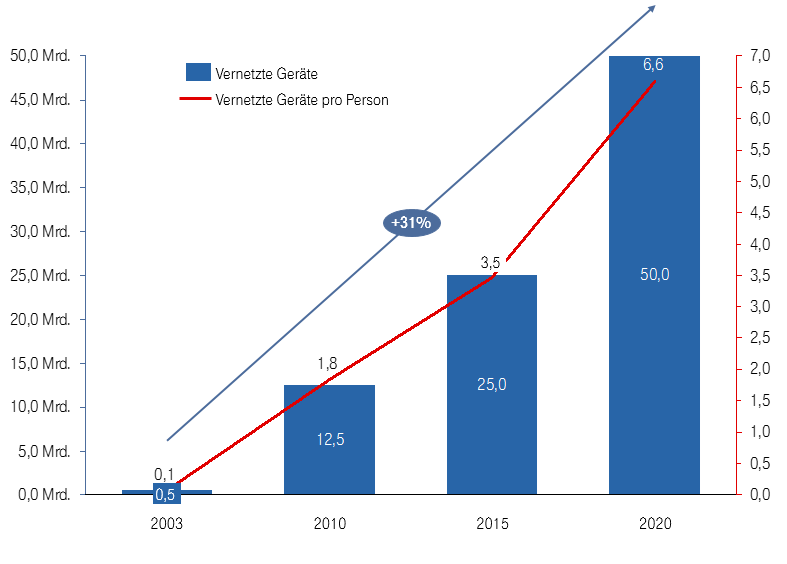
\includegraphics[width=0.8\textwidth]{Entwicklung_Anzahl_vernetzte_Geraete}
	\caption{Die Entwicklung der Anzahl vernetzter Geräte}
	\label{fig:Entwicklung_Anzahl_vernetzte_Geraete}
\end{figure} 

Zunehmend werden immer mehr physikalische Objekte mit Mikrokontrollern, Sendeempfängern und geeigneten Protokollen für digitale Kommunikation ausgestattet. Dadurch steigt die Anzahl der mit dem Internet verbundenen Geräte, was Abbildung 1 illustriert. Prognostiziert ist, dass sich die Anzahl der mit dem Internet verbundenen Geräte bis zum Jahr 2020 auf 50 Milliarden erhöhen wird. Auf die Weltbevölkerung umgerechnet bedeutet das, dass jeder Mensch 6,6 vernetzte Geräte besitzen wird (siehe Abbildung 1). Mit diesem Durchbruch auf dem ITK-Markt entstehen neue Datenmengen, die früher noch nicht vorhanden waren. Diese Datenmengen müssen über Telekommunikationsnetze übertragen werden. Dadurch werden die Zugangsnetze und insbesondere die Kernnetze der Telekommunikationsanbieter stärker denn je belastet.  
Ein zweiter Trend der heutigen Informationsgesellschaft ist die rasant wachsende Nachfrage nach Bandbreite. Diese entsteht durch die Konvergenz von Medien und Telekommunikation. Orts- und zeitunabhängige TV-Nutzung, Video on Demand, Pay TV und HD sind beispielsweise treibende Faktoren für den Konsum von Bandbreite. 
Telekommunikationsnetze sind buchstäblich die Basis des täglichen Lebens und müssen mit immer mehr Datenverkehr umgehen können. In der logischen Konsequenz werden in Zukunft mehr Netzkomponenten verwendet, um den Anforderungen der vielen vernetzten Geräte und der Breitbandnachfrage gerecht zu werden. Das bedeutet auch einen Anstieg des Energieverbrauchs für die Betreibung der Telekommunikationsnetze. Bereits 2012 verbrauchten die herkömmlichen Rechenzentren in Deutschland jährlich über zehn Terawattstunden Strom, was etwa der Leistung von zwei Kernkraftwerken des Typs Brunsbüttel entspricht. Die wachsende Bevölkerung, der Klimawandel und die Verknappung der Energieressourcen stehen somit im starken Zielkonflikt. Eine Herausforderung ist es daher, die Telekommunikationsnetze umwelt- und ressourcenschonend zu gestalten. 



\section{Stand der Forschung} \label{SdF}
Definition Wirtschaftlichkeit, Carriernetz
Betriebskosten, Wirtschaftlichkeit, etc.
CAPEX OPEX
Wirtschaftlichkeit
Definieren
Wir betrachten einen Teil der Betriebskosten, nämlich: .....
% Evtl. die Sachen zu Wirtschaftlichkeit mit einem Hinweis, dass wir uns auf einen Teil, nämlich die Betriebskosten beschränken, in entweder Problemstellung oder Methodik

\subsection{Begrifflichkeiten}
Wirtschaftlichkeit
Bei der Betrachtung von Energieeinsparpotentialen in Netzwerken ist der Begriff der Wirtschaftlichkeit von Bedeutung. Allgemein bedeutet Wirtschaftlichkeit den sinnvollen und sparsamen Einsatz vorhandener Mittel. Wirtschaftlich handelt, wer eine gegebene Leistung mit einem minimalen Ressourceneinsatz erreicht. Das Prinzip des minimalen Einsatzes von Ressourcen zum Erbringen einer Leistung wird Minimalprinzip genannt []. Bezogen auf Einsparpotentiale in Netzwerken bedeutet Wirtschaftlichkeit den minimalen Einsatz von Energie in Form von Strom zum Betreiben eines Netzwerks.


Carrier-Netzwerke
Gegenstand der Projektarbeit bildet ein hinsichtlich der Energieeffizienz und Wirtschaftlichkeit zu optimierendes Carrier-Netzwerk.
Unter einem Carrier versteht man […] eine Gesellschaft, die mindestens drei Übertra\-gungs\-wege betreibt, die über eine Vermittlungsstelle miteinander verbunden sein müssen"' (aus: \cite{carrier}). Ein Carrier-Netzwerk stellt somit physikalische Transportwege und -verfahren zur Verfügung und bildet die Grundlage für sogenannte Value Added Services von Providern, welche auf den Carrier-Diensten aufsetzen \cite{fassnacht}. "`Bei den TK-Transportwegen unterscheidet man leitergebundene Verbindungen auf der Basis von Kupferkabeln oder Lichtwellenleitern sowie Funkverbindungen wie Satellitenverbindungen, Richtfunkstrecken und Rundfunkverbindungen"' (Aus: Ebd.).%TODO: Zitat korrigieren

Somit umfasst ein Carrier-Netzwerk nicht nur das physikalische Backbone-Netz, sondern auch das Zugangs- und Aggregationsnetzwerk. Im Rahmen des Projektes entfällt die Betrachtung der Optimierungspotentiale des Zugangsnetzes zugunsten einer aus\-führ\-lich\-eren Simulation von wirtschaftlichen und energieeffizienten Netzkonzepten im Backbone- und Aggregationsnetzwerk. So bildet der Broadband Network Gateway (BNG) die niedrigste Netzelementebene. Multi-Service Access Nodes (MSAN), Digital Subscriber Line Access Multiplexer (DSLAM), enhanced NodeBs (eNodeB) und weitere Netzelemente der nächsttieferen Hierarchiestufe fallen somit aus der Betrachtung.


Betriebskosten (OpEx – operating expenditures) 
Für die Wirtschaftlichkeitsbetrachtung des Netzwerks werden die Ausgaben für die Anschaffung der Netzwerkkomponenten (Capex –Capital Expenditures) nicht berücksichtigt. Die für den operativen Geschäftsbetrieb anfallenden Aufwendungen werden „Operating Expenditures“ (kurz Opex) genannt. Zu den laufenden Ausgaben für den Geschäftsbetrieb gehören u.a. Mieten, Personal- und Energiekosten, Aufwendungen für Wartung und Support, Verbrauchsmaterialien und Betriebsstoffe. 
Die Betrachtung der Wirtschaftlichkeit beschränkt sich auf einen Teil der Kosten für den operativen Betrieb, nämlich auf die Kosten für Energie zum Betrieb der Netzelemente.


\subsection{Möglichkeiten und Konzepte zur Reduzierung des Energieverbrauchs}
%Evtl mit dem nächsten Subchapter zusammenlegen? Hier nicht schreiben über unsere Simulation. Es geht nur darum, was andere schon erforscht haben.
Aufgrund des prognostizierten Datenverkehrs, den öffentlichen Diskussionen zur Nachhaltigkeit und Klimawandel, sowie den steigenden Energiekosten für Netzbetreiber, kommt dem Thema Energieverbrauch in Telekommunikationsnetzen immer mehr Aufmerksamkeit zu. Laut der ETH Zürich liegt die zukünftige Wachstumsrate des Internetstromverbrauchs zwischen 4 und 7 Prozent jährlich. [QUELLE]. Damit liegt die Steigerung des Energieverbrauchs für den Betrieb des Internets über dem Wachstum des weltweiten Gesamtstromverbrauchs (jährlich circa 3,5 Prozent in den letzten Jahren.  Die Entwicklung und Anwendung von Energieeinspartechnologien können demnach den stetig wachsenden Kosten für Betrieb der Netzelemente entgegenwirken. 
Die gesamtheitlichen Kosten der Telekommunikationsnetze der Carrier lassen sich in OpEx (Aufwendungen für Stromverbrauchskosten) und CapEx (Aufwendungen für Anschaffung der Netzkomponenten, Investitionen für unterbrechungsfreie Stromversorgungen usw.) einteilen. In typischen Betriebsstellen beträgt der Energiebedarf für den Betrieb unterbrechungsfreier Stromversorgungen und Kühlung der Netzwerkelemente etwa 50 Prozent des Gesamtenergiebedarfs [QUELLE]. Damit besteht hier ein großes Einsparpotenzial. Bezüglich des reinen Telekommunikationsnetzes können Möglichkeiten zur Steigerung der Energieeffizienz bzw. Reduzierung des Energieverbrauchs wie folgt unterteilt werden:
\begin{itemize}
	\item Energieeffiziente Netzelemente: Durch den technologischen Fortschritt können Netzwerkkomponenten energieeffizienter gestaltet werden wie z.B. durch zunehmende Integration einzelner Module. Somit können mehrere Module in einer Einheit zusammengefasst werden ohne die Netzwerkarchitektur zu verändern. 
	\item Energieeffiziente Netzarchitektur: Beim Entwerfen von Netzarchitekturen kann durch das Einbeziehen des Energieverbrauchs eine Reduzierung des Gesamtenergieverbrauchs bewirkt werden.  Die Verwendung unterschiedlicher Netzzugangsarchitekturen hat verschiedene Energieverbräuche zur Folge (z.B. Fiber to the Home gegenüber Fiber to the Building).
	\item Verkehrslastadaptiver Netzbetrieb: Bei dem zuvor erwähnten zunehmenden Datenverkehr und dem entsprechenden Netzausbau, führt eine nahezu konstante Leistungsaufnahme der Netzelemente zu einem Anstieg des Netzenergiebedarfs. Da jedoch die Verkehrslast des Netzes zeitlich variiert [Quelle], können in Phasen geringerer Last einzelne Systeme in einem Modus mit niedrigerer Leistungsaufnahme betrieben werden, ohne dass eine Beeinträchtigung für die Nutzer entsteht. Heutige Telekommunikationsnetze werden auf Basis einer Spitzenlast zuzüglich einer Reserve dimensioniert. Für die Dimensionierung der Netze stellt eine dynamische Anpassung der Netzkapazität an die Verkehrslast eine attraktive Lösung dar. [QUELLE]
\begin{figure}[!]
	\centering
	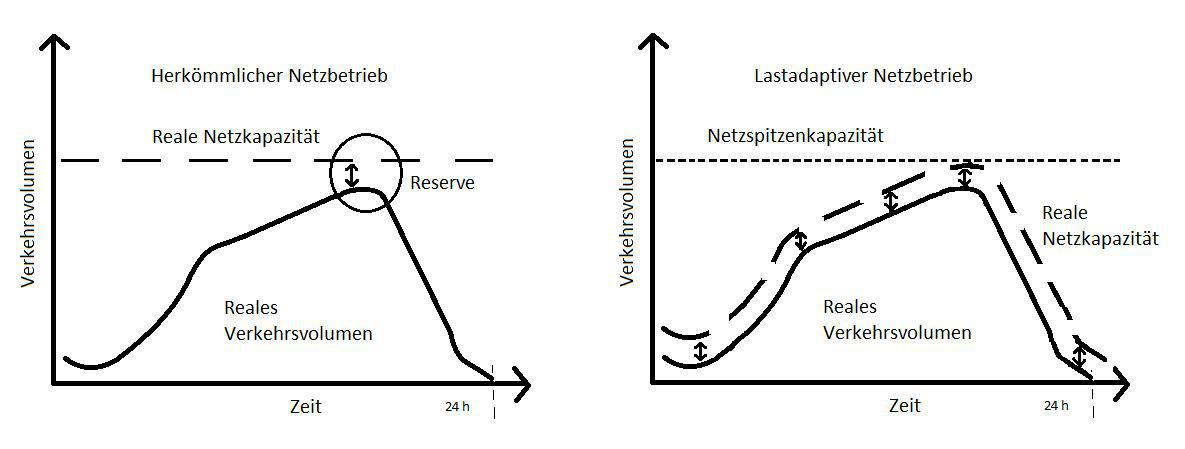
\includegraphics[width=0.8\textwidth]{Netzdimensionierung}
	\caption{Prinzipien der Netzdimensionierung}
	\label{fig:Netzdimensionierung}
\end{figure}
Der linke Teil dieser Abbildung zeigt den Netzbetrieb, dessen Kapazität aufgrund einer Spitzenlast zuzüglich einer Reserve dimensioniert wurde. Es ist erkennbar, dass die reale Netzkapazität auf einen Tag verteilt nur einmal annähernd erreicht wird. Je geringer der Abstand zwischen der Funktion der realen Netzkapazität und dem Graphen ist, desto effizienter ist das Netz. Durch die statische Netzkapazität ist ein konstanter Energieaufwand notwendig, um das Netz zu betreiben. Im rechten Teil der Abbildung ist dargestellt, wie durch den lastadaptiven Netzbetrieb ein effizienteres Netz gestaltet werden kann. Die reale Netzkapazität passt sich dem realen Verkehrsvolumen an und dessen Verläufe sind bis auf eine vorgehaltene Reserve gleich. Betrachtet man beide Teile der Grafik ist zu erkennen, dass der Abstand der Gerade und dem Graphen beim lastadaptiven Netzbetrieb um einige Vielfache geringer ist als bei dem statisch dimensionierten Netz. Somit ist das Netz um einige Vielfache effizienter. 
\end{itemize}



\begin{equation}
P_{core} = P_{ip} + P_{ethernet} + P_{otn} + P_{wdm}
\end{equation}


\subsection{Energie-effiziente Technologien}
Das zweite Konzept befasst sich mit der dynamischen Abschaltung von temporär nicht verwendeten Netzwerkkomponenten und setzt das Konzept des lastadaptiven Netzbetriebs um.  Tageszeitabhängige Schwankungen der Netzauslastung ermöglichen eine unabhängige und dynamische Abschaltung von Ports und Links unter der Berücksichtigung der Quality of Service-Bedingungen [2]. Dabei werden Algorithmen zur Identifikation von individuell abschaltbaren Links verwendet [10]. Die Verfasser W. Fisher, M. Suchara und J. Rexford schreiben in ihrer Veröffentlichung „Greening Backbone Networks: [...]“, dass die durchschnittliche Verbindungsauslastung der Backbone-Netzwerke vieler großer Internet Service Provider geschätzt 30-40\% beträgt. Durch die Abschaltung einzelner Ports kann laut der Deutschen Telekom AG der Energiebedarf einiger Elemente um ein Drittel gesenkt werden [Energieverbrauch in Tele.... C.Lange ...]. Demnach verbrauchen Ports die, keinen Verkehr leiten signifikant weniger Energie als solche unter Last. Weiterhin wird beschrieben, dass durch die Deaktivierung ganzer Line Cards und Port Groups per Management Systems nahezu 100\% Einsparung erreicht werden kann. In dem Text von 2010 wird beschrieben, dass das Deaktivieren der Line Cards nur per manuellen Eingriff mit einem Network Management System erfolgen kann [.... C.Lange]. Der Aufwand für das dynamische, temporäre Abschalten steht nicht im Verhältnis zur Einsparung. Die Hersteller der Backbone-Netzwerk-Komponenten implementieren derzeit Funktionen, die das manuelle Eingreifen durch eine automatische Kapazitätsanpassung ersetzen. Die Herausforderung in den nächsten Jahren wird zum einen sein die Deaktivierungs- und Aktivierungszeiten der Elemente zu reduzieren. Weiterhin ist es notwendig die Betriebssysteme großer Router Systeme für die genannte Dynamik kompatibel zu machen, da aktuelle Softwarelösungen eine temporäre Aus- und Abschaltung nicht vorsehen.


Bei den Technologien beschränkt sich die Arbeit auf optische Vermittlungstechniken. Optische leitungsvermittelnde Switche basieren auf mikro-elektromechanischen Systemen, die eine geringe Menge an Energie benötigen und eine hohe Portanzahl besitzen. Das sog. Hybrid Optical Switching (HOS) verwendet eine Kombination aus optischen und elektronischen Netzknoten. Zum einen verwendet HOS das „Optical Circuit Switching“ (OCS), das laut C. Xin, C. Qiao, Y. Ye und S. Dixit in der Veröffentlichung „A Hybrid Optical Switching Approach“ als fortgeschrittene und viel verwendete Technologie zur Übermittlung in optischen Netzwerken eingesetzt wird. OCS ist gut geeignet für langanhaltende und kontinuierliche Datenströme, jedoch kommt die Technik bei stoßweisen Anstieg des Durchsatzes an ihre Grenzen. Eine alternative Technologie stellt „Optical Burst Switching“ (OBS) dar. Wie der Name darlegt ist die Technologie optimiert für kurzzeitig ansteigende Datendurchsätze. Ein Nachteil der Technik ist die abnehme Leistung bei lang andauernden, kontinuierlichen Strömen. Weiterhin stellt OBS eine hohe Bandbreitennutzung her, benötigt hierfür aber große optische Pufferspeicher. Um effektiv beide Varianten der Datenströme zu übertragen, können mit der Kombination von OCS und OBS die Vorteile beider Technologien kombiniert werden. Die beiden Technologien sind als komplementäre Ansätze anzusehen. [Xin, C. Qiao, Y. Ye und S. Dixit]. In einem HOS-Netzwerk werden große Datenströme durch vorgehalten Leitungen oder mit langen Durchsatzstöße übertragen und kleinere Ströme durch einzelne Datenpakete und kurze Durchsatzstöße übermittelt.


\section{Problemstellung}
Wie oben beschrieben existieren bereits einige Möglichkeiten, den Energieverbrauch in Carrier-Netzwerken zu senken. Allerdings werden diese Möglichkeiten noch nicht umfänglich in realen Netzwerken umgesetzt. Ein denkbarer Grund für diesen Rückstand realer Backbone-Netze sind wirtschaftliche Bedenken der Netzbetreiber. Im Folgenden wird die Motivation für Netzbetreiber beschrieben, den Energieverbrauch ihrer Netze stärker zu berücksichtigen, sowie die Ziele dieser Arbeit.
%citation needed!

\subsection{Motivation}
Obwohl der Stromverbrauch der OECD-Staaten seit mehreren Jahren stagniert oder sogar leicht zurück geht, wachsen die globalen Verbräuche weiter an (vgl. Abbildung \ref{fig:ProbStromSektor}). Dies kann vor allem auf  Schwellenländer zurückgeführt werden, die in kurzer Zeit ein rasantes wirtschaftliches Wachstum erleben.

\begin{figure}[!ht]
	\centering
	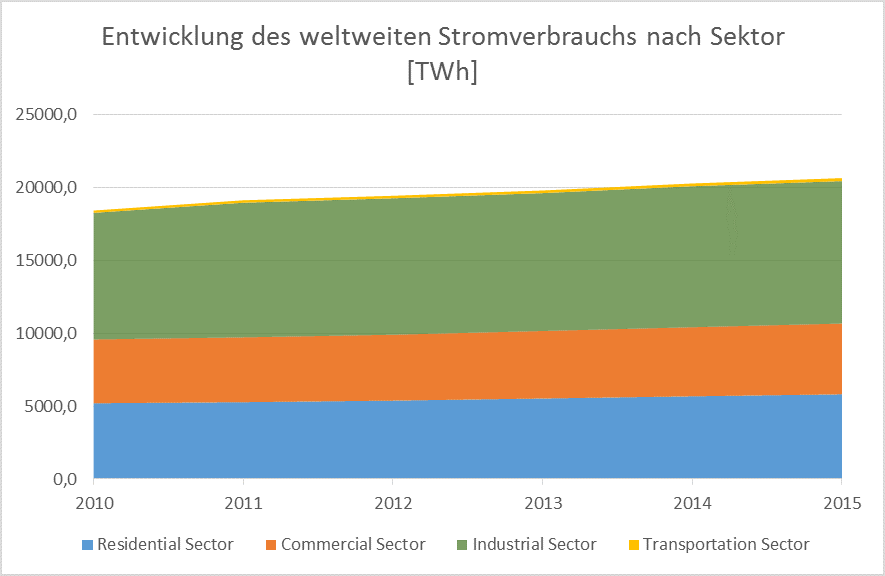
\includegraphics[width=0.8\textwidth]{ProbStromSektor}
	\caption{Weltweiter Stromverbrauch nach Sektoren, basierend auf \cite{bibid}}
	\label{fig:ProbStromSektor}
\end{figure}
Da aller Bemühungen zum Trotz die fossilen Energieträger Erdöl, Kohle und Erdgas weiterhin ca. 81\% der weltweiten Energieerzeugung ausmachen \cite{statista} und diese Ressourcen nicht regenerierbar sind, sind langfristig steigende Energiekosten (\cite{iea2015}, S. 40f) ein großes Risiko für ICT-Provider weltweit, die insgesamt mit steigenden Kosten zu kämpfen haben.

Steigende Energiekosten für sich genommen wären schon ein starkes Argument, Netze effizienter zu gestalten.  Der Effekt der Kosten wird allerdings potenziert durch den Fakt, dass der Stromverbrauch von ICT von 2007-2012 stärker gewachsen ist als der globale Stromverbrauch (vgl. \cite[9]{vanhedde}). Schon 2012 betrug der Anteil von ICT am globalen Stromverbrauch etwa 5\% (s. Abbildung \ref{fig:ProbStromICT})

\begin{figure}[!ht]
	\centering
	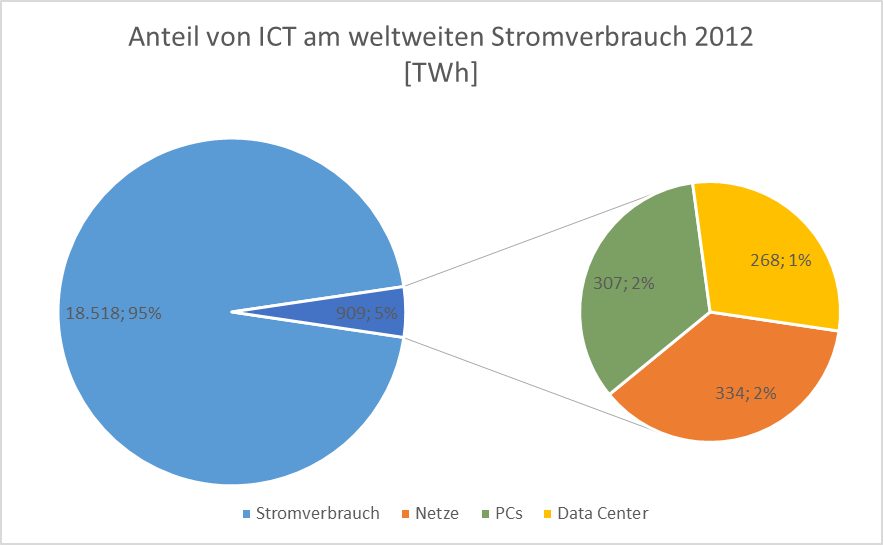
\includegraphics[width=0.8\textwidth]{ProbStromICT}
	\caption{Anteil von ICT am weltweiten Stromverbrauch, basierend auf \cite{bibid} und \cite{bibid}}
	\label{fig:ProbStromICT}
\end{figure}

Seit dem ist der Anteil der Bevölkerung weltweit, der das Internet verwendet, von 20,6\% (2007) auf 43,4\% (2015) gestiegen \cite{itu}. Dieses Wachstum wird sich in der nächsten Zukunft nicht verlangsamen. Weiterhin sorgen steigende Datenvolumen pro Nutzer für eine wachsende Netzlast. Welchen Effekt die Industrie 4.0 und das Internet of Things auf die Netze weltweit haben werden, lässt sich momentan  noch nicht abschätzen. Eins jedoch steht fest: Das Netz der Zukunft wird mehr Daten zu bewältigen haben als jemals zuvor.
%evtl. nach oben ziehen als 1. Absatz für Problemstellung

\subsection{Ziele}
Das Ziel der vorliegenden Arbeit ist es, abzuschätzen, wie viel Energie bzw. Kosten  durch Verwendung energieeffizienter Technologien eingespart werden können.

Zur Erreichung dieses Ziels ist zum einen eine Literaturrecherche zu den bestehenden Technologien nötig, die es ermöglichen, den Energieverbrauch von Netzen zu senken. Die Ergebnisse dieser Literaturrecherche befinden sich in Kapitel \ref{SdF}.

Es soll eine Software entwickelt werden, die es ermöglicht, zwei hypothetische Netze miteinander zu vergleichen, zum einen ein konventionelles Netz, wie es heutzutage Stand der Technik ist, zum anderen ein energieeffizientes Netz, das die vorhandenen Technologien und Konzepte zur Effizienzsteigerung sinnvoll einsetzt. Anhand des abgeschätzten Energieverbrauchs der beiden Netze wird das Energiesparpotenzial sowie die möglichen Kosteneinsparungen durch den Betrieb des energieeffizienten Netzes ausgegeben. Die Ergebnisse der Softwareentwicklung sowie die Abschätzung des Energieverbrauchs befinden sich in Kapitel \ref{Ergebnisse}.

Die Softwarelösung wird als objektorientierte Java Desktop Anwendung mit einer Einteilung der Klassen in die drei Bereiche Model, View und Controller implementiert.

Der Prozess der Softwareentwicklung soll nach dem Wasserfallmodell ablaufen. Die Programmaufteilung und geforderte Funktionen sind bereits vor der Implementierung hinreichend bekannt, so dass die Anwendung eines agilen Entwicklungsmodells hier keine entscheidenden Vorteile bietet. Das genaue Vorgehen in der Softwareentwicklung wird im folgenden Kapitel erläutert.

\section{Vorgehen}

\subsection{Modellierung}
Zwei Netze modelliert (Quellen), um sie gegenüberstellen zu können. Techniken aus Kapitel "Energieeffiziente Technologien" eingesetzt.
Aufgrund der Recherche ist Simulation nötig.

\subsection{Softwareentwicklung}
Die zuvor beschriebene Modellierung zur Kalkulation und Simulation von energieeffizierten Netzen soll im nächsten Schritt softwaretechnisch umgesetzt werden. Als Vorgehensmodell hat sich das Projektteam an dem Wasserfallmodell mit den folgenden Entwicklungsstufen orientiert:
\begin{itemize}
\item Anforderungsanalyse
\item Spezifikation
\item Systemdesign
\item Programmierung / Implementierung
\item Test
\end{itemize}
Die Analyse der Anforderungen an die Simulationssoftware erfordert eine zielgerichtete Recherche über bereits vorhandene Technologien und Methoden. Ebenfalls müssen die Funktionalitäten, die das Simulationstool bereitstellen soll, abgegrenzt werden. Die Anforderungen werden zunächst als Ideen und Möglichkeiten gesammelt und dann in Form von Anforderungsspezifikationen definiert. 
Das System soll ein statisches Netz mit einer festgelegten Anzahl an Verbindungen abbilden. Alle Daten zu Geräten, Netzen, Verbindungen und Netzprofilen sollen in einer MySQL-Datenbank gespeichert werden. Die Verwendeten Geräte sowie neue Netzprofile sollen über die Datenbank eingepflegt werden können. Für das Netzprofil sollen Traffic-Daten (Netzprofil, Last, Quelle, Senke, Uhrzeit) verwendet werden. Aus den Daten entsteht eine gleichbleibende Auslastungskurve, anhand dessen die Verbindungen für die jeweilige Uhrzeit definiert werden können. Um das Netz möglichst realistisch zu simulieren bekommen die einzelnen Verbindungen eine Länge zugeordnet. Anhand dieser Länge (mehr als 80 km) wird definiert, ob ein Verstärker hinzugefügt werden muss, um die Verbindung zu verbessern. Das definierte, statische Netz soll die Verwendung verschiedener Technologien und Methoden zur Senkung des Energieverbrauchs möglich machen. Zur Abschaltung von Switches und Ports soll ein Algorithmus entwickelt werden, der auf dem „Exhaustive Greedy Algorithm“(QUELLE!!!) aufbaut.
Im Zuge der Anforderungsanalyse und der Spezifikation der Software wurden die folgenden funktionalen, nicht funktionalen und datenbezogenen Anforderungen erstellt:



Funktionale Anforderungen:
\begin{itemize}
	\item A1: Über die Datenbank kann ein Netz, bestehend aus Knoten (Geräte) und Kanten (Verbindungen) modelliert werden
	\item A2: Das Anlegen neuer Geräte und Gerätekonfigurationen ist über die Datenbank möglich
	\item A3: Das Verändern von Geräteparametern ist über die Datenbank möglich
	\item A3a: Das Austauschen von Gerätetypen ist über die Datenbank möglich
	\item A3b: Das Austauschen von Gerätetypen pro Schicht ist über eine GUI möglich                       
	\item A4: Das System berechnet anhand des modellierten Netzes, der eingestellten		 Gerätekonfigurationen, der gewählten Energiespartechnologien und des vorliegenden Lastprofils den Stromverbrauch.
	\item A5: Das System berechnet die Stromkosten anhand des Stromverbrauches und einem vorgegebenen Umrechnungsfaktor 
	\item A6: Zur Vereinfachung von Berechnungen müssen Annahmen getroffen werden, die in der DB hinterlegt werden
	\item A7: Es werden generische Geräte basierend auf dem Dokument "<Dokumentname einfügen>" verwendet
	\item A8: Zur Abschaltung von Switches/Ports dient der "Exhaustive Greedy Algorithm"
	\item A9: Der simulierte Stromverbrauch im Laufe eines Tages soll pro Stunde graphisch ausgegeben werden
	\item A10: Die Lastkurve wird graphisch dargestellt
\end{itemize}


Nicht funktionale Anforderungen:
\begin{itemize}
	\item NFA1: Das System soll als Client-only Applikation vorliegen
	\item NFA2: Das System verwendet eine MySQL-Datenbank als Persistenzschicht
\end{itemize}


Datenbezogene Anforderungen:
\begin{itemize}
	\item DA1: Verbindungen wird eine Länge zugewiesen
	\item DA2: Für Gerätetypen können relevante Leistungs- und Verbrauchsparameter hinterlegt werden
	\item DA3: Ein Netz entsteht durch das Verbinden von Geräteinstanzen und der Zuordnung zu einer NetzID
	\item DA4: Annahmen werden durch einen eindeutigen Namen und einen Wert abgebildet
	\item DA5:  Die Netzlast wird in Form von Datenpaketen mit den Attributen Volumen, Quelle, Senke, Uhrzeit, Profil-ID definiert
\end{itemize}


In der Systemdesign-Phase werden einige Entscheidungen bezüglich der Softwareentwicklung getroffen. Als Programmiersprache für das Projekt wurde objektorientiertes Java ausgewählt. Die bereits vorhandene Entwicklungserfahrung im Team mit dieser Sprache und der sehr ausgeprägten Verfügbarkeit von kostenfreien Entwicklungstools und fertigen Bibliotheken waren für die Entscheidung ausschlaggebend.
Die Architektur besteht aus einer 2-Tier Kombination aus einer relationalen MySQL/MariaDB Datenbank und einer Fat-Client Anwendung. Die Datenbank wird dabei zur Speicherung der zur Erstellung eines Netzes notwendigen Daten, sowie Hardware-, Topologie- und Netzwerkkonfiguration verwendet. Die Anwendung hingegen wird zur Parameterkonfiguration, Berechnung der Zielwerte und Ausgabe der Resultate verwendet.
Die Vorteile dieser Architektur sind die gute Portabilität der resultierenden Lösung und die Ermöglichung einer einfachen und schnellen Entwicklung. Es müssen keine weiteren Anwendungsserverkomponenten je Entwicklungsumgebung installiert und konfiguriert werden. Die SQL-Datenbank verwendet eine übliche Datenbank-Standardsoftware und kann per SQL-Script vollautomatisch konfiguriert werden.
Das Datenbank-Konzept ist entscheidend für die Softwareentwicklung. Es werden alle relevanten Daten für Berechnungen, Konfigurationen und Darstellungen gespeichert. Auf der Basis der Datenbankstruktur kann die Entwicklung der Softwarelösung weitergeführt werden.


\begin{figure}[!]
	\centering
	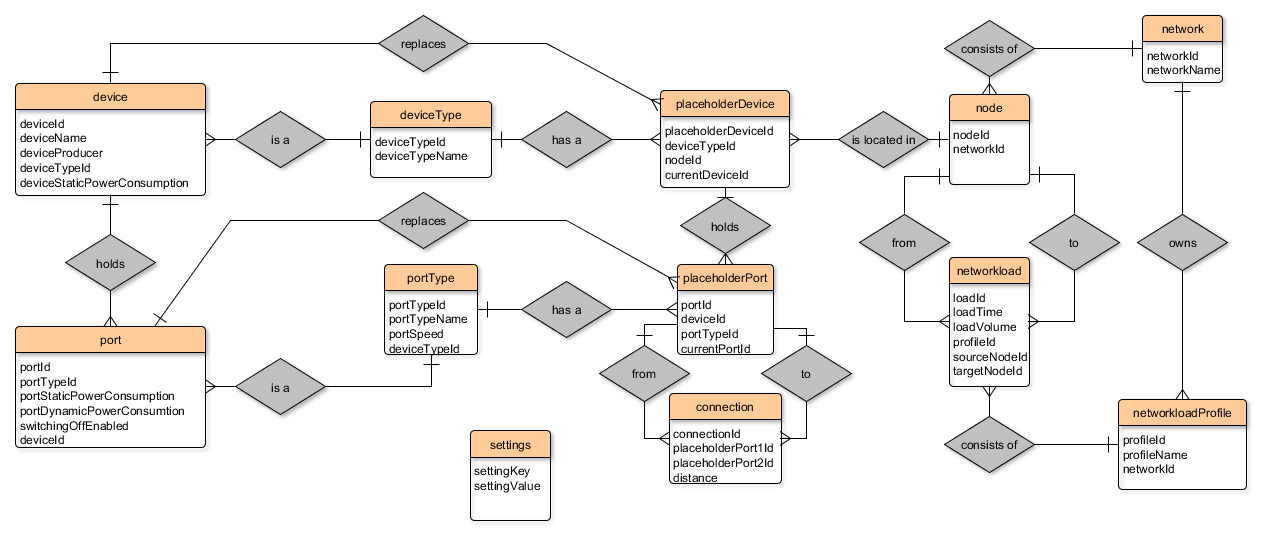
\includegraphics[width=0.8\textwidth]{MethSoftwareER}
	\caption{ER-Diagramm} %TODO Bezeichnung anpassen
	\label{fig:MethSoftwareER}
\end{figure}


%----> Erklärung ER-Diagramm <----
Zur Vorbereitung der Programmierung wurde der Algorithmus für das Routing in der Systemdesign-Phase entwickelt.  Dieser Algorithmus wird in den nächsten Kapiteln (4.3 \& 5.1) detailliert erklärt.
In der Programmierungsphase wurde ein Grundgerüst für die weitere Entwicklung der Software geschaffen. Die Datenbank wurde auf der Basis des zuvor erstellten Konzeptes eingebunden. Im Rahmen der Weiterentwicklung kann der Routing-Algorithmus und die definierten Anforderungen implementiert werden. Der Algorithmus koordiniert das Routing des Traffics durch das definierte Netz. Mit der Hilfe von weiteren Annahmen und Algorithmen kann die Software zu einem System entwickelt werden, das verschiedene Technologien und Methoden zur Energiereduzierung einsetzt. Das Programm könnte die verschiedenen Methoden möglichst realitätsgetreu anwenden und die dadurch gesparte Energie graphisch darstellen. Über die GUI könnte eine Konfiguration möglich sein.  Darüber könnten verschiedene Technologien aktiviert und Geräte ausgetauscht werden. 
Die beschriebene Software konnte innerhalb dieses Projektes nicht fertigstellt werden. Gründe dafür waren die Begrenzung der Bearbeitungszeit auf drei Monate und vermehrt auftretende komplexe Problemstellungen. Die einzelnen Faktoren der Komplexität werden in Kapitel 4.4 erläutert.
Eine ausgereifte Testphase ist erst nach der Fertigstellung der Software sinnvoll. Die implementierten Module und Teilfunktionalitäten werden vom jeweiligen Entwickler direkt getestet. Ein abschließender Test der bis zum Ende der Bearbeitungszeit programmierten Funktionalitäten, wird durchgeführt.


Implementierung

%TODO
TODO wohin mit dem folgenden Abschnitt?
Um den Energieverbrauch im Carrier-Netzwerk berechnen zu können, bedarf es an Werten der im Backbone verwendeten Netzkomponenten. Innerhalb der Simulation wird für die Berechnung des Gesamtverbrauchs auf die definierten Werte zurückgegriffen, die in einer Datenbank gespeichert sind. Ziel dieser Arbeit ist die Simulation und Berechnung des gesamtheitlichen Energieverbrauchs. Deshalb verwendet die Berechnung die von den beiden Wissenschaftler Ward Van Heddeghem und Filip Idzikowski in ihrer Veröffentlichung \cite{vanhedde} zusammengetragenen Werte. Die Quelle beinhaltet zum einen das analytische Model der Berechnung und zum anderen ein Datenblatt \cite{vanhsheet} des Energieverbrauchs der unterschiedlichen Hersteller. Das Datenblatt gliedert die Geräte nach den Unterschiedlichen Layer IP/MPLS, Ethernet, OTN, WDM - (OSI-Layer: 3-2-1-1). Zu beachten ist beim Verwenden der Werte, dass es sich um Werte unter typischen Lastbedingungen handelt, die sich nach der Kapazität der Komponente richtet und nicht nach dem aktuellen Durchsatz. Des Weiteren geben die Werte nur dein Stromverbrauch für den Betrieb an, ein Verbrauch für Kühlung o.Ä. ist nicht enthalten.
Der Gesamtverbrauch des Core-Networks ergibt sich aus der Summe alle Verbrauche der einzelnen Schichten.

\subsection{Entwicklung des Routing-Algorithmus}\label{subsec:MethAlg}
Zur Simulation des Netzwerkes, der Lastverteilung und des elektrischen Stromverbrauches des Netzwerkes ist ein iteratives Berechnen für einzelne Zeitabschnitte abhängig von der Netzlast, des Traffic-Ursprungs und des Traffic-Ziels notwendig.

Es stehen zur Berechnung des Stromverbrauchs je Zeitabschnitt generell mehrere Ansätze zur Verfügung. Der einfachste Ansatz wäre je Uhrzeit von einer bestimmten zuvor als Datenbankeintrag festgelegten Nutzungsauslastung je Verbindung auszugehen. Dies würde ein einfaches Bestimmen der einzelnen Geräteauslastungen und anschließendem addieren der Werte zu einem Gesamtstromverbrauch pro Zeiteinheit ermöglichen. Diese Ergebnisse könnten dann als Tabelle und Histogramm dargestellt werden.

Dieser Lösungsweg setzt allerdings eine sehr detaillierte und statische Modellierung eines Beispielnetzes und allen dazugehörigen Auslastungs- und Verbrauchswerten je Zeitabschnitt voraus. Aufgrund dieses Konfigurationsaufwands wird ein Anwender folglich einen großen Zeitraum je Iteration auswählen, was zu einer sehr groben und realitätsfernen Simulation führen würde. Energiespartechniken wie das dynamische Abschalten von einzelnen Verbindungen und umrouten der Netzlast auf andere noch nicht optimal ausgelastete Verbindungen muss der Anwender in diesem Verfahren selbstständig je Iteration umsetzen.

Eine weitere Möglichkeit zur Berechnung der optimalen Stromverbrauchswerte bietet das automatisierte, in einem Algorithmus implementierte Berechnen der einzelnen Netzlast-Routing-Möglichkeiten und anschließend der Wahl des nach zuvor definiertem Regelsatz besten routings. Dieser Algorithmus bietet den Vorteil, dass der Anwender nur die Netzlast mit Iterationszeitraum, Quelle, Senke und Menge spezifizieren muss und die Software daraus selbstständig die beste oder eine gute Lösung errechnet.
Dies erlaubt allerdings keine Anpassung des zu berechnenden N


\subsection{Komplexität bei der Entwicklung}
Die Komplexität, die Unterschätzung der Einflussfaktoren und deren Beziehung zueinander werden häufig zu Problemen der Softwareentwicklung. In diesem Projekt konnte die Komplexität der Umsetzung der Aufgabenstellung erst in der Realisierungs- / Programmierungsphase erkannt werden. Im Zuge der Anforderungsanalyse und Spezifikation wurden Anforderungen definiert, die ein automatisiertes und konfigurierbares System zur Berechnung und Darstellung von energieeffizienten Netzen beschreiben. Während der Umsetzung der Anforderungen wurden komplexe Problemstellungen entdeckt, die erfasst und nach der Auswirkung auf das Projekt bewertet wurden. Bei dem Versuch diese Probleme zu lösen oder zu umgehen, sind weitere komplexe Schwierigkeiten aufgetaucht. Aufgrund von zwei Faktoren wurde die Entwicklung der Software bei einem Grundgerüst belassen. Ein Mangel an Ressourcen machte es nicht möglich, die auftauchenden komplexen Problemstellungen genau im System abzubilden. Daher mussten Annahmen getroffen werden, die die Genauigkeit der vom System erwarteten Ergebnisse stark reduzierte. Da ungenaue Ergebnisse in diesem Forschungsgebiet nicht zielführend und akzeptabel sind, wurde die Software nicht entsprechend der zuvor definierten Anforderungen weiter entwickelt. Die Komplexität der Entwicklung soll im Folgenden detailliert beschrieben werden.  


Die Implementierung eines Netzes bedarf einem Lastprofil, mehreren Geräten und der jeweiligen Verbindung zwischen zwei Geräten. Der in Kapitel 4.3 beschriebene Algorithmus soll das Routing durch das Netz pro Zeitintervall berechnen. Ein Zeitintervall soll unterschiedlich einstellbar sein. Es muss sichergestellt werden, dass keine Verbindungen überlastet sind. Dafür muss der Algorithmus zunächst die optimale Route berechnen und diese dann mit allen bereits definierten Verbindungen vergleichen. Wurde die gleiche Verbindung bereits gewählt muss geprüft werden, ob die Geräte der Verbindung voll ausgelastet sind. Ist die maximale Auslastung erreicht, muss entschieden werden, welche Verbindung bestehen bleibt und für welche Verbindung eine alternative Route gefunden werden muss. Dies kann nur über eine komplizierte Berechnung und einen Vergleich durch den Algorithmus durchgeführt werden. Ein weiteres Problem beim Routing ist die Blockierung der Ports. In der Realität werden Ports nur eine bestimmt Zeit belastet. Diese Zeit ist abhängig von der Datenmenge und Geschwindigkeit des Ports. Die Berechnung der Zeit, die ein Port von einem Datenpaket blockiert wird, macht  die Verwendung von festen Zeitintervallen fast unmöglich. Es müsste  definiert werden, wie lange der Port mit welchem Volumen belegt ist. Dadurch würden die Zeitschlitze zur kleinsten Einheit. Um diese Komplexität zu minimieren wurde die Annahme getroffen, dass ein Datenpaket einen Port für die gesamte Zeiteinheit belegt.

 
Eine weitere Annahme musste bei der Berechnung des Stromverbrauchs getroffen werden. Jedes Gerät besitzt einen vom Hersteller vorgegebenen Stromverbrauch pro Port. Der Stromverbrauch für das gesamte Gerät ergibt sich nicht aus der Multiplikation von Stromverbrauch pro Port und der Anzahl an Ports. Der Grund dafür ist, dass das Gerät auch Strom verbraucht, wenn kein Datenpaket über die Leitung geht. Daher ist der genaue Stromverbrauch bei heruntergefahrenen Ports nur ungefähr abschätzbar. Des Weiteren muss der Stromverbrauch für Geräte, die sich im Energiesparmodus befinden, geschätzt werden. Zu dieser Problematik kommt noch die Komplexität der Berechnung des Stromverbrauchs des gesamten Netzes dazu. Mit heruntergefahrenen und in der Geschwindigkeit reduzierten Ports und Geräten, muss zu jedem Zeitpunkt der Status des jeweiligen Ports und Geräts bekannt sein.  


\section{Präsentation und Auswertung der Ergebnisse} \label{Ergebnisse}
\subsection{Algorithmus} \label{subsec:ErgAlg}
% Hier bitte neutral den Algorithmus beschreiben (Pseudocode in Worte umsetzen)
Grundlegend ist das Ziel, für jeden Zeitabschnitt die beste erzielbare Lösung zur stromsparenden Bewältigung (Durchleitung) des Traffic von dem Eingangspunkt in das Netz (Quelle) bis zum Austrittspunkt (Senke) zu berechnen. Zur Vereinfachung wurde die Annahme getroffen, dass Über die Dauer eines Zeitabschnittes (einer Iteration) die durch den Algorithmus getroffene Routing-Entscheidungen und die Wahl der abzuschaltenden Hardware gleich bleiben. Diese werden je Iteration initial einmal neu berechnet. Durch die Verkürzung der Iterationsdauer und der dazu passenden Netzlast-Daten lässt sich bei geringem Aufwand ein genaueres, verfeinertes Modell durchrechnen, so dass ein realistischeres Resultat zu erwarten ist.


\begin{figure}[!]
	\centering
	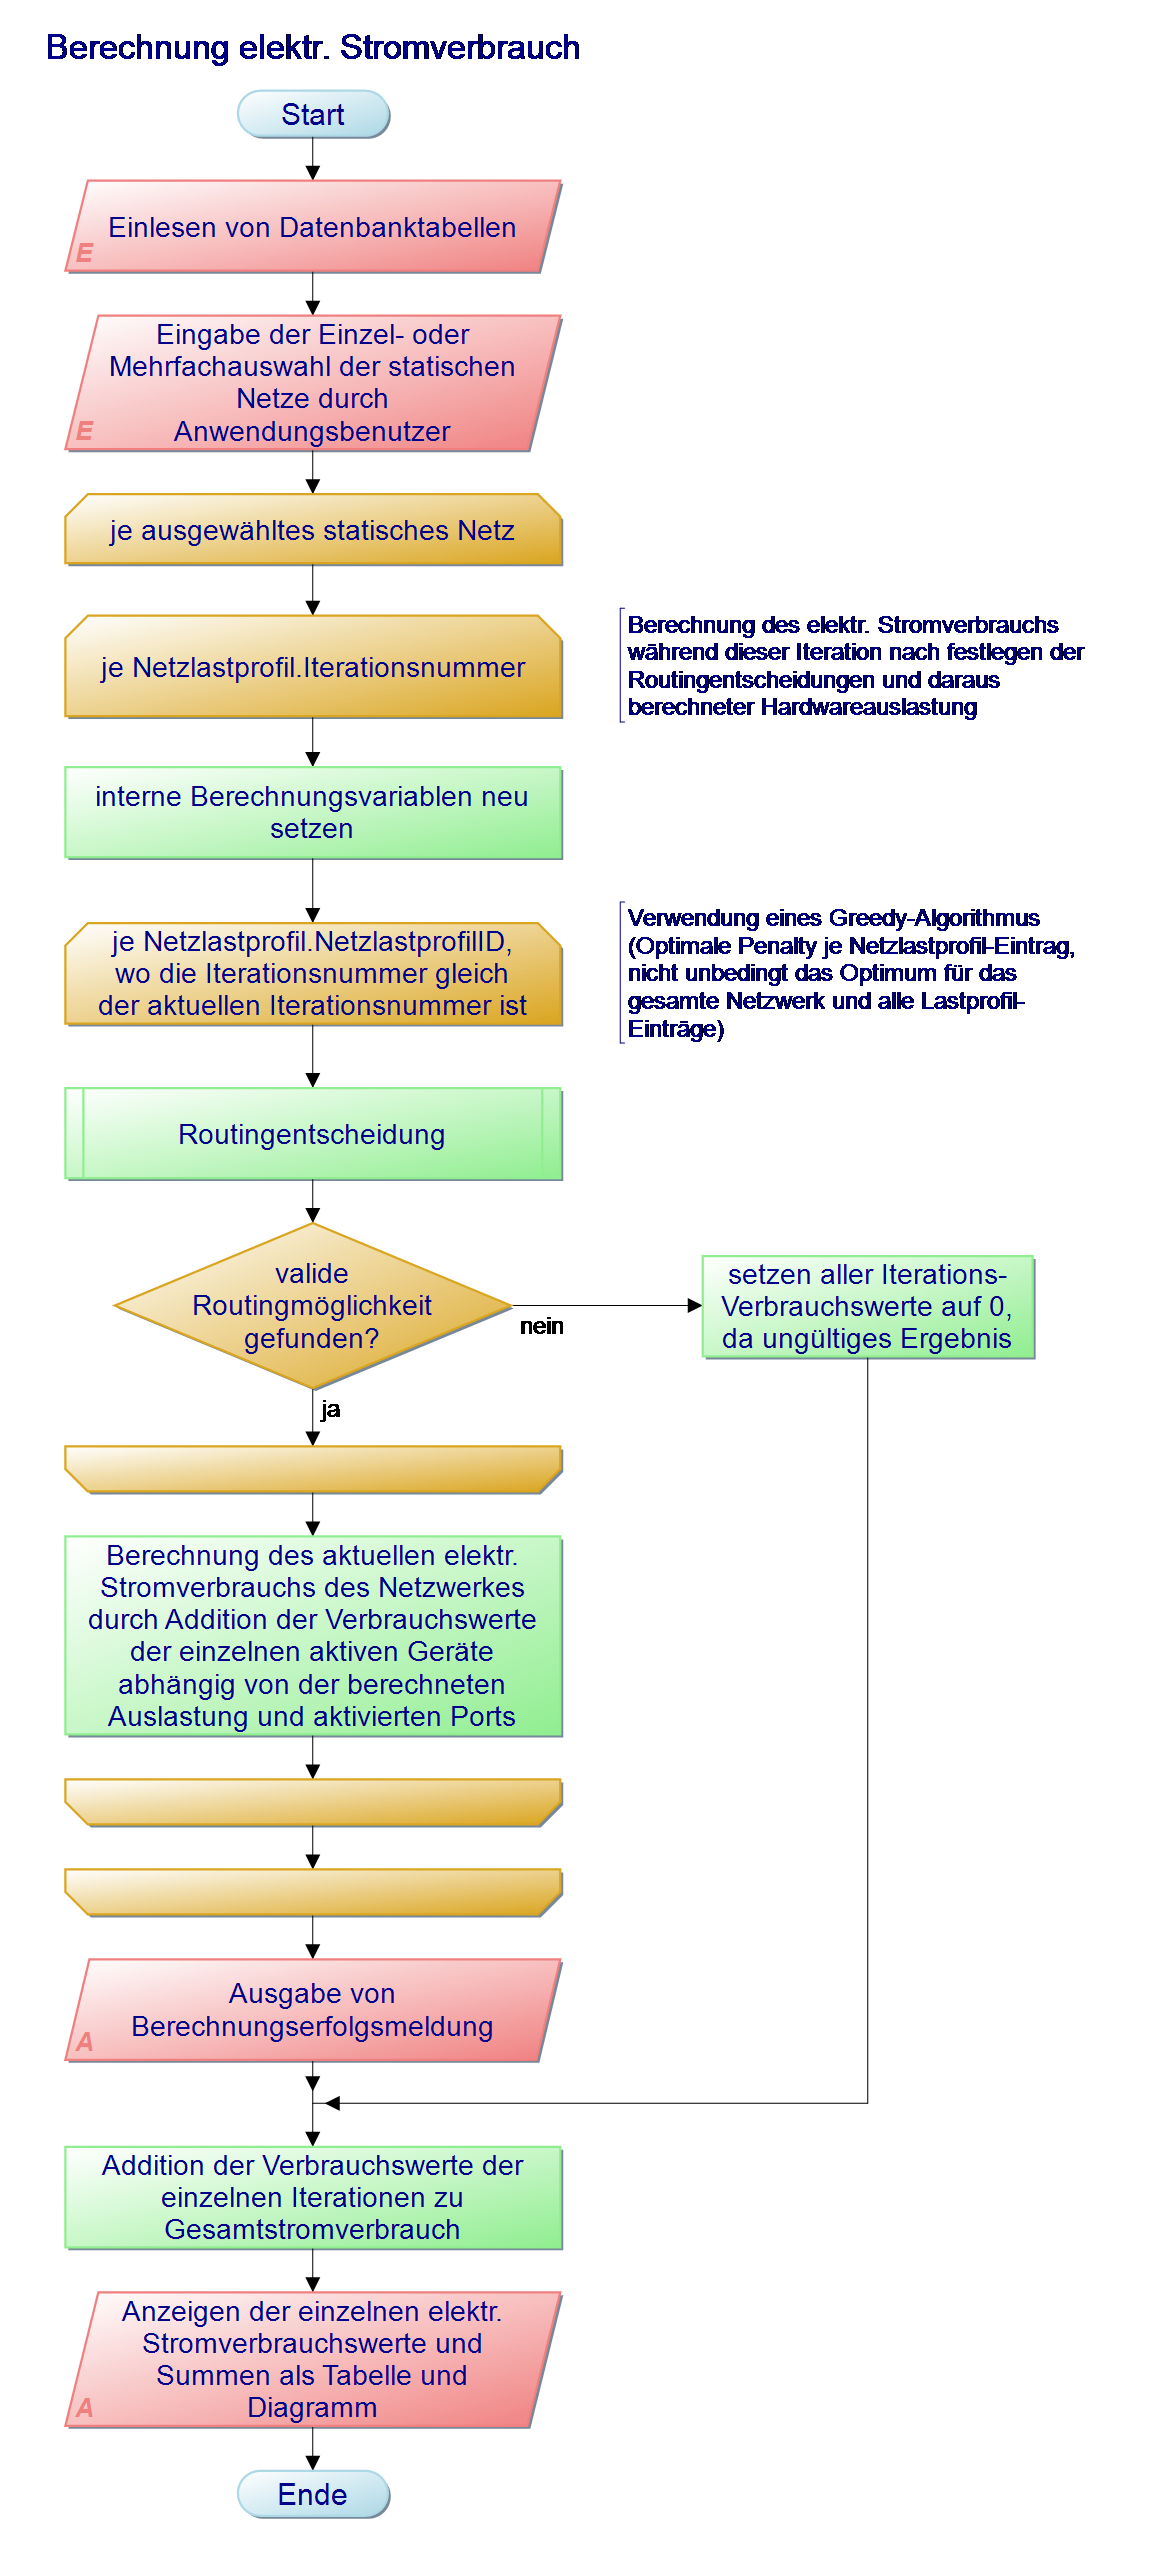
\includegraphics[width=0.6\textwidth]{1Berechnung_elektr_Stromverbrauch}
	\caption{Programmablaufplan zur Anwendungslogik}
	\label{fig:1Berechnung_elektr_Stromverbrauch}
\end{figure}


Je durch den Anwender in der Datenbank hinterlegtem statischen Netz wird eine Datenreihe bestehend aus einem Stromverbrauchswert je Iterationszeitraum berechnet.
Um diese Einzelwerte zu berechnen, werden zuerst die Lasten aus jedem Netzlastprofil-Eintrag auf möglichst effizient auf die Netzwerkhardware und Verbindungen projiziert, und danach abschließend abhängig von den berechneten Geräteauslastungen die Teil-Stromverbrauchswerte addiert.


Mit dieser groben Vorgehensweise lässt sich das gesuchte Ergebnis je Modellnetzwerk inklusive dem zeitlichen Verlauf errechnen. Allerdings fehlt dazu noch die Antwort auf die Frage, wie die effizienten Routing-Entscheidungen getroffen werden können. Der folgende Teil des Algorithmus beschreibt eine möglichen Lösung:


Um zu entscheiden, welches Routing für die einzelnen Netzlastprofil-Einträge je Iteration das beste Resultat liefert, wird je mögliche Route eine dynamische Penalty (Kosten-Faktor) berechnet. Anschließend wird für das Netzlastprofil die Route mit der niedrigsten errechneten Penalty, welche die Datendurchsatzgrenzen der Hardware und somit der einzelnen Verbindungen nicht überschreiten, als beste Route angenommen. Diese Kategorie von lokalen Lösungsverfahren nennt man Greedy Algorithmus. Dieser liefert nicht unbedingt das insgesamt beste Ergebnis, sondern berechnet nur das lokale Optimum für das betrachtete Teilproblem. Um eine schnelle praktische Ausführungszeit auch bei Berechnungen mehrerer Vergleichsnetze mit kurzen Iterationsintervallen zu erreichen beinhaltet dieser Algorithmus intelligente Entscheidungsfunktionen um schlechte Routen frühzeitig zu ignorieren und nicht zielführende Berechnungen wie sie beispielsweise bei Schleifenbildung auftreten zu verhindern.
\begin{figure}[!]
	\centering
	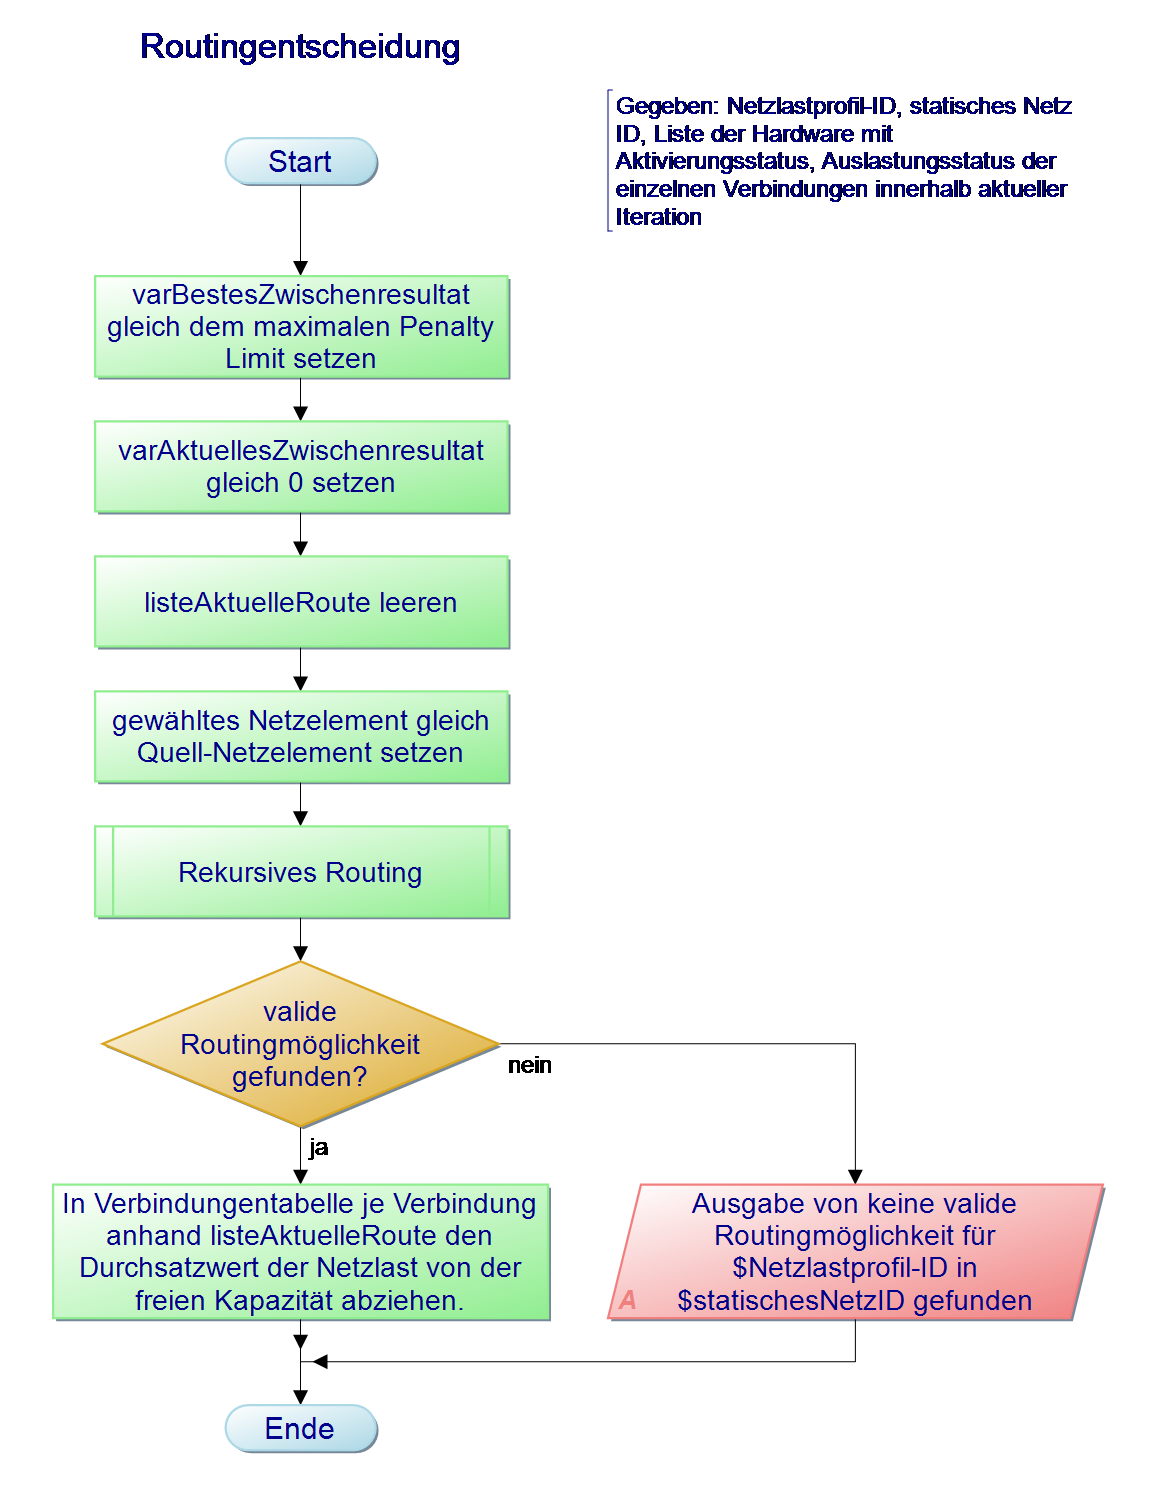
\includegraphics[width=0.6\textwidth]{2Routingentscheidung}
	\caption{Programmablaufplan zum übergreifenden Anteil des Routing-Algorithmus}
	\label{fig:2Routingentscheidung}
\end{figure}

Da die zur Verbindungsbewertung verwendete Penalty mehreren Faktoren wie Latenz, elektr. Stromverbrauch, Kapazität der Verbindung und auch An-/Aus-Status der Hardware berücksichtigen muss, und diese einzelnen Faktoren je nach Verwendungszweck des Netzes unterschiedliche Gewichtung haben, müssen die einzelnen Anteile mit vom Anwender der Simulationssoftware festgelegten Gewichtungsfaktoren multipliziert werden. Damit kann der Nutzer die Netzsimulation auf seine Anforderungen ansatzweise anpassen.
\begin{figure}[!h]
	\centering
	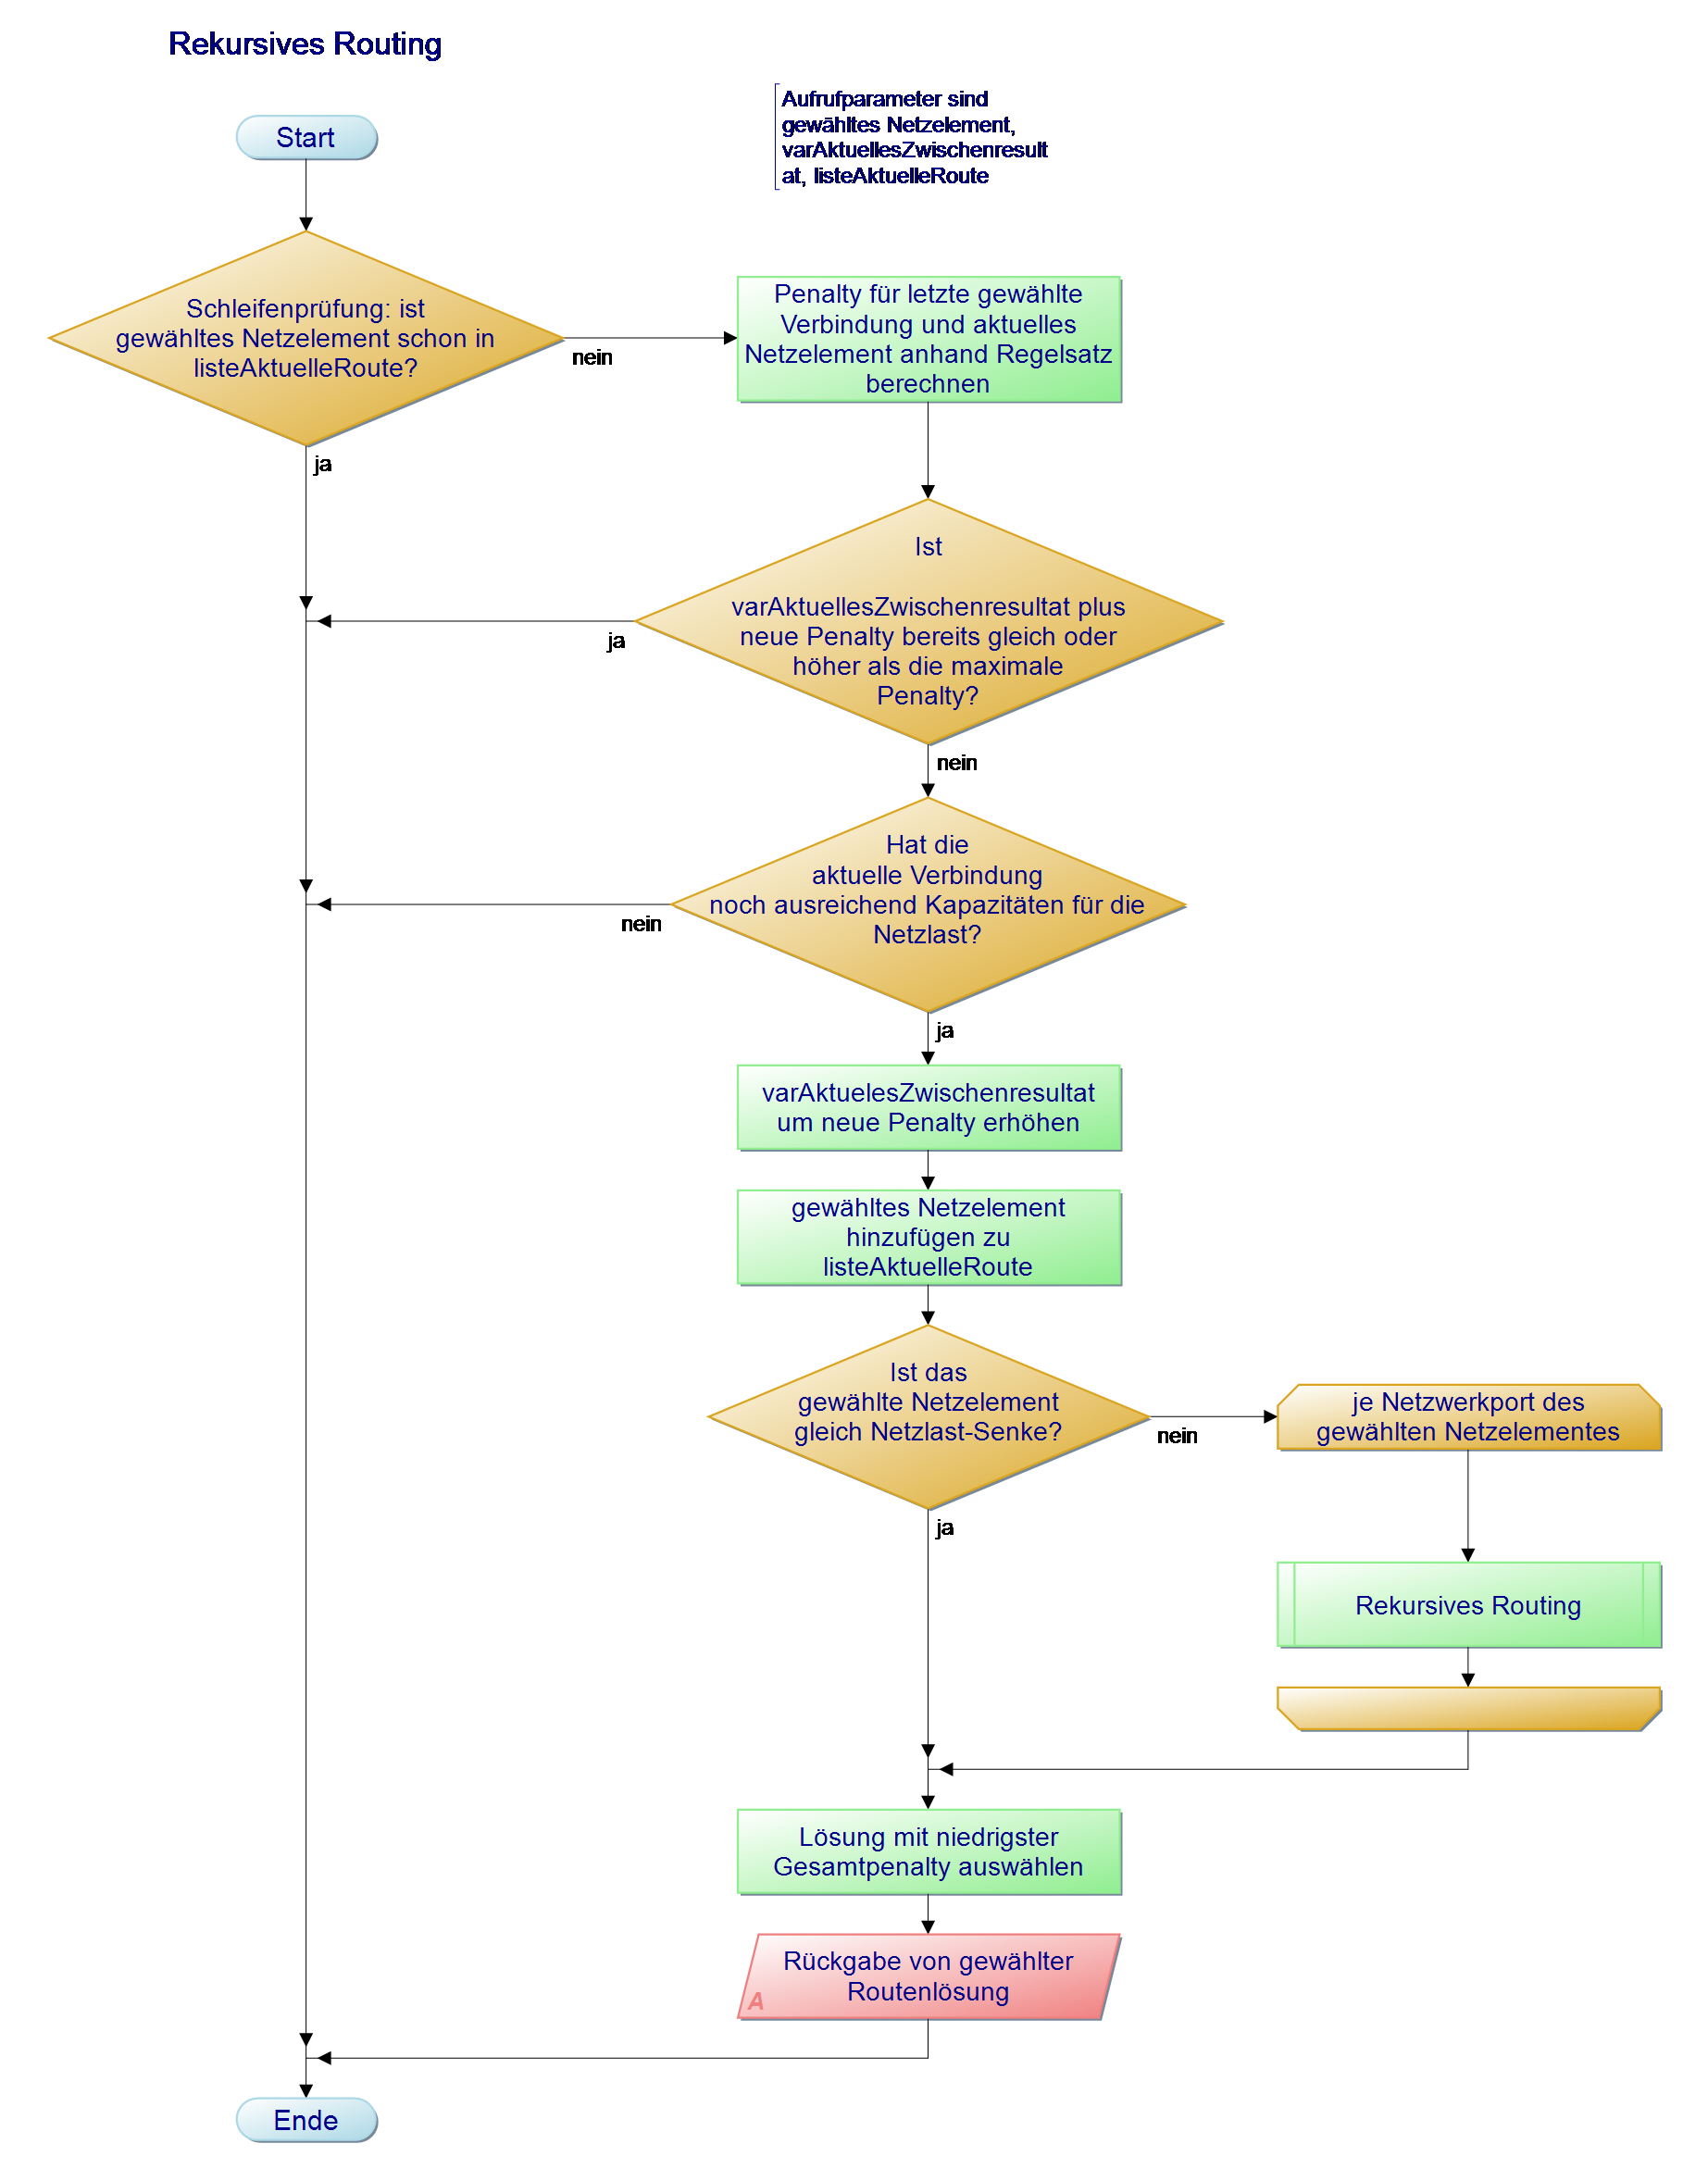
\includegraphics[width=0.6\textwidth]{3Rekursives_Routing}
	\caption{Rekursiver Anteil des Routing-Algorithmus}
	\label{fig:3Rekursives_Routing}
\end{figure}


Alles in allem ist ein Regelsatz zur Penaltyberechnung je Iteration notwendig, an Hand welchem die Algorithmus-Implementierung jeweils versucht das lokale Optimum zum Routingproblem als Lösung zu finden.
Der folgende Regelsatz stellte sich beim logischen durchspielen einer solchen Simulation als Grundlage heraus:
\begin{itemize}
	\item Zum Anfang jeder neuen Iterations-Zeitphase sind alle Geräte und alle Ports soweit diese dies unterstützten ausgeschaltet
	\item Das Aktivieren eines Devices kostet Penalty (hoch)
	\item Das Aktivieren eines Ports kostet Penalty (niedrig)
	\item Das Ausschalten des Port-Energiesparmodus kostet keine Penalty, um vermeidbares aktivieren anderer Hardware / Ports zu vermeiden. Energiesparmodus-Capability zählt lediglich zur Berechnung des Stromverbrauchs.
	\item Um niedrige Paketlaufzeiten durch das Netz sicherzustellen, kostet jeder Hop / genutzte Verbindung eine weitere Penalty (hoch)
\end{itemize}
Einzelne Verbindungen haben zusätzlich zu dem dynamischen Anteil außerdem jeweils eine feste Penalty basierend auf Verstärkeranzahl + Länge -> statischer Wert in Datenbank.

% Diskussion des Ergebnisses und der Schwierigkeiten bei der Implementierung werden im nächsten Kapitel berücksichtigt

%TODO: getroffene Annahmen und Verallgemeinerungen erläutern

\subsection{Die erstellte Software aus Ergebnissicht}
Im Rahmen der Software-Entwicklung wurde das Java-Programm „EnergyNetSim“ mitsamt Anbindung an eine MySQL-Datenbank realisiert. Die folgenden Unterkapitel beschreiben die erzielten Resultate und geben Hinweise auf Installation und Benutzung der Software für Endanwender.

\subsubsection{Ergebnisse der Software-Entwicklung}
Die erstellte Software „EnergyNetSim“ stellt ein Rahmenwerk zur Verfügung, in das die in den Kapiteln
\ref{subsec:MethAlg} und \ref{subsec:ErgAlg} beschriebenen Algorithmen zur Simulation von Netzauslastung, Datenverkehr zwischen zwei Netzknoten, dynamischem Routing und effizienzsteigernden Energiesparmechanismen eingefügt werden können. Im Programmcode und in der Dokumentation sind die dazu notwendigen Methoden bereits angelegt und gekennzeichnet. Das Kapitel \ref{sec:ErgSoftwErweiterung} gibt dazu detailliertere Hinweise.
Aufgaben wie die Selektion der zu betrachtenden Netze, die einfache Adaption von Parametern zur Simulation, die persistente Speicherung der Konfigurationen und Netzstrukturen und die graphische Ausgabe der errechneten Ergebnisse übernimmt der aktuelle Softwarestand bereits. Die Grundlage dafür bietet die Einbindung der frei verfügbaren Java-Bibliothek „jFreeChart“\footnote{„JFreeChart is a free 100\% Java chart library that makes it easy for developers to display professional quality charts in their applications. JFreeChart's extensive feature set includes, a consistent and well-documented API, supporting a wide range of chart types; a flexible design that is easy to extend,[…] support for many output types, including Swing and JavaFX components, image files (including PNG and JPEG).[…] JFreeChart is open source or, more specifically, free software. It is distributed under the terms of the GNU Lesser General Public Licence (LGPL), which permits use in proprietary applications.“ \cite{jdbc}} und des offiziellen JDBC-Treibers\footnote{Frei verfügbar unter https://dev.mysql.com/downloads/connector/j/5.1.html} zur Verbindung mit der MySQL-Datenbank.
\begin{figure}[!ht]
	\centering
	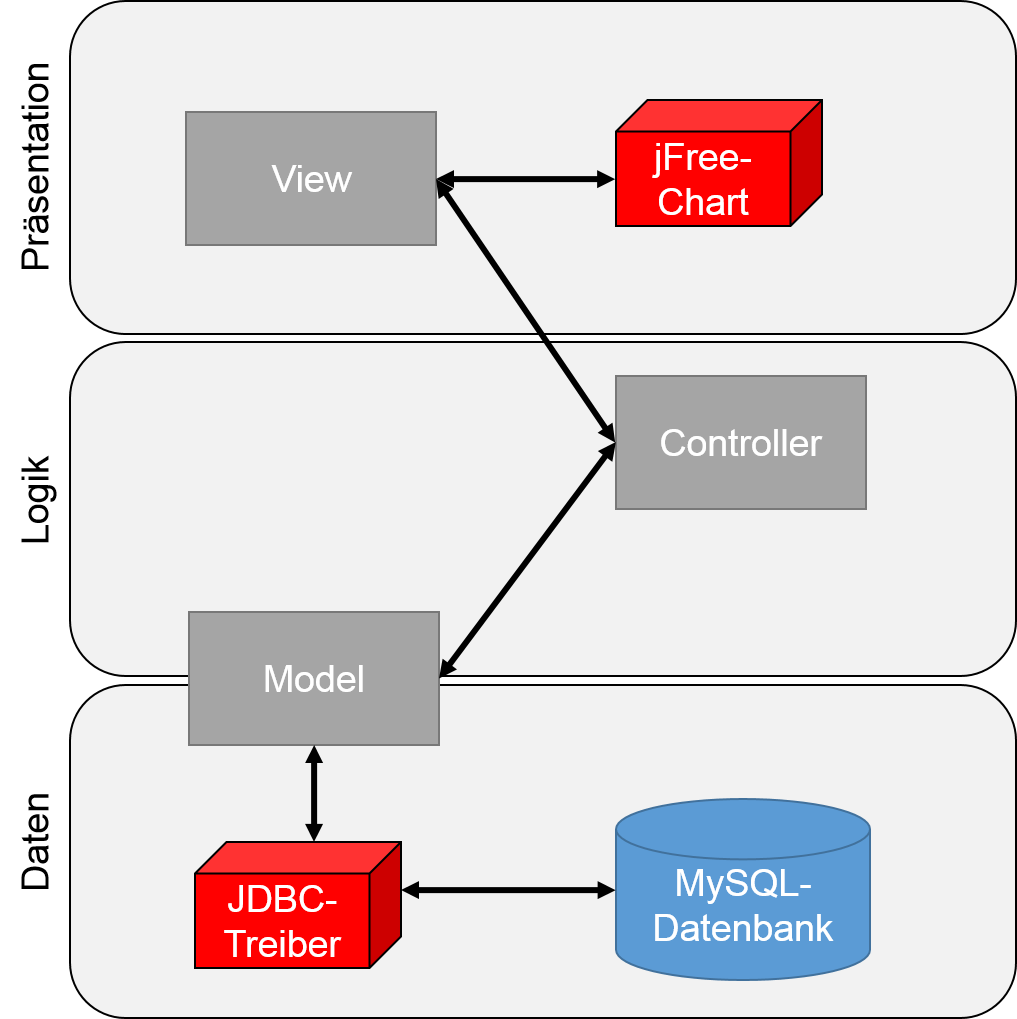
\includegraphics[width=0.5\textwidth]{ErgSoftwareMVC}
	\caption{Schichtenarchitektur des EnergyNetSim (eigene Darstellung)}
	\label{fig:ErgSoftwareMVC}
\end{figure}
Das Zusammenspiel zwischen Java-Anwendung und der MySQL-Datenbank zeigt
Abbildung \ref{fig:ErgSoftwareMVC}. Bei der Entwicklung wurde ein „Model-View-Controller“ (kurz: MVC)-Entwurfsmuster gewählt, das die Trennung der Programmstruktur in die logischen Schichten „Datenhaltung“, „Programmlogik“ und „Präsentation“ ermöglicht.
Das Programm wird mitsamt den Datenbank-Skripten zur Erstellung der Datenbankstrukturen auf zwei Arten zur Verfügung gestellt:
\begin{itemize}
\item Als offenes Repository „EnergyNetSim/Simulator.git" über den Versionsverwaltungsdienst GitHub: https://github.com/EnergyNetSim/Simulator.git
\item Als ausführbares Java-Archiv (JAR), das in der Anlage zum vorliegenden Bericht enthalten ist.
Auf die notwendigen Schritte zur Installation der erstellten Software wird im nachfolgenden Kapitel eingegangen.
\end{itemize}

\subsubsection{Installation der Software}
Von den zwei vorgestellten möglichen Wegen, über die Simulationssoftware zu beziehen ist, wird im Anschluss die Inbetriebnahme mittels JAR-Datei beschrieben. Das Kapitel richtet sich somit vornehmlich an Endanwender.
Die Einbindung des GitHub-Repositories ist vor allem für Entwickler interessant und erfordert daher Kenntnisse im Umgang mit der Versionsverwaltungssoftware Git, einer zusätzlichen Java-Entwicklungsumgebung, beispielsweise IntelliJ oder Eclipse. Des Weiteren muss das Java-Development-Kit in seiner aktuellsten Version installiert werden. Was gerade in Kurzform skizziert wurde, würde in einer ausführlichen Fassung den Rahmen des Berichts sprengen. Außerdem existiert eine ausreichende Zahl an Online-Communities und Anleitungen\footnote{Auf der Webseite von GitHub findet sich eine Sammlung von Links zum Erlernen von Git: https://help.github.com/articles/good-resources-for-learning-git-and-github/
Ebenso bietet Oracle eine ausführliche Java-Dokumentation: http://www.oracle.com/technetwork/java/javase/downloads/index.html} zur Verwendung der beschriebenen Programme, sodass aus einer erneuten Schilderung kein wissenschaftlicher Mehrwehrt entstünde.
Bis das Java-Programm mittels JAR-Datei ausgeführt werden kann, sind die in Abbildung \ref{fig:ErgSoftwareInst1} abgebildeten Schritte erforderlich.
\begin{figure}[!ht]
	\centering
	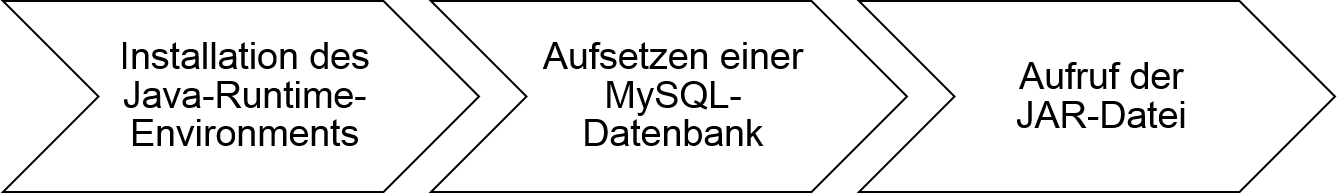
\includegraphics[width=0.8\textwidth]{ErgSoftwareInst1}
	\caption{Schritte der Installation}
	\label{fig:ErgSoftwareInst1}
\end{figure}
Voraussetzung ist das Vorhandensein der aktuellsten Version der Java-Laufzeitumgebung, kurz „JRE“. Innerhalb dieser Umgebung kann die Anwendung betriebssystemunabhängig in der Java-Virtual-Maschine (kurz: „JVM“) ausgeführt werden. Das Java Runtime Environment ist über die Webseite der Firma ORACLE\footnote{Zum Zeitpunkt der Abgabe des Berichtes ist der Download über folgenden Link möglich: http://www.oracle.com/technetwork/java/javase/downloads/jre8-downloads-2133155.html} zu beziehen und zu installieren.
Weil die Java-Anwendung auf eine MySQL-Datenbank als Persistenzschicht zugreifen soll, wird zusätzlich ein lokaler MySQL-Server benötigt, der über die IP-Adresse 127.0.0.1 / „localhost“ und den Port 3306 erreichbar ist. Das Entwicklerteam empfiehlt den Einsatz des Open-Source-Datenbankservers „MySQL Community Server“, der ebenfalls von ORACLE\footnote{Zum Zeitpunkt der Abgabe des Berichtes ist der Download über folgenden Link möglich: http://dev.mysql.com/downloads/mysql/} unter der GNU General Public License kostenlos angeboten wird. Ebenfalls empfehlenswert ist die Verwendung des Datenbank-Modellierungs- und Manipulationswerkzeugs „MySQL Workbench“, das über denselben Weg bezogen werden kann.
Nach der erfolgreichen Installation der beschriebenen Komponenten muss der SQL-Server gestartet werden, um die Datenbank anzulegen. Für Nutzer eines Windows-Betriebssystems sind dazu folgende Schritte erforderlich:

\begin{description}
\item [Starten des MySQL-Server-Dienstes:]
Durch Klick auf „starten“ wird der SQL-Server hochgefahren und der Status ändert sich in „Gestartet“.
\begin{figure}[!ht]
	\centering
	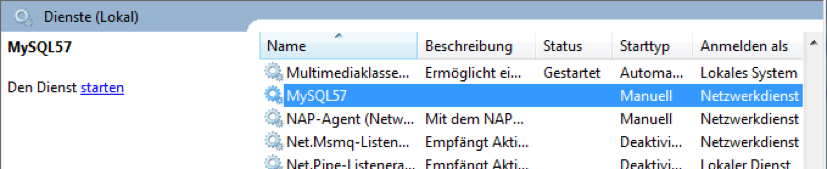
\includegraphics[width=0.8\textwidth]{ErgSoftwareInst2}
	\caption{Starten des MySQL-Server-Dienstes}
	\label{fig:ErgSoftwareInst2}
\end{figure}
\item [Anlegen einer neuen Verbindung zum Server:]
Innerhalb der MySQL-Workbench wird eine Verbindung zum MySQL-Server mit den in Tabelle \ref{tab:mysql} aufgeführten Daten hergestellt.
\begin{table}[htp!]
\centering
	 \begin{tabular}{|l|l|l|}
	 \hline
	Parameter & Wert\\
	\hline
	\hline
	Connection Method & Standard (TCP/IP)\\
	 \hline
	Hostname & 127.0.0.1\\
	 \hline
	Port & 3306\\
	 \hline
	Username & root\\
	 \hline
	Passwort & Wird bei der Installation angezeigt\\
	 \hline
	 \end{tabular}
\caption{Parameter für das Einrichten des DB-Verbindung in der MySQL Workbench}
\label{tab:mysql}
\end{table}
\begin{figure}[!ht]
	\centering
	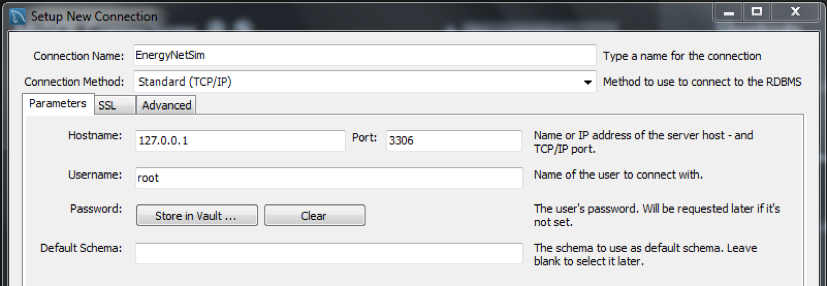
\includegraphics[width=0.8\textwidth]{ErgSoftwareInst3}
	\caption{Konfigurieren einer neuen Verbindung zum MySQL-Server}
	\label{fig:ErgSoftwareInst2}
\end{figure}
\item [Importieren des Datenbank-Schemas:] Das Initialisierungsskript der Datenbank, welches sich im Anhang des Projektberichts angehängt ist, kann daraufhin über Server > Import Data > Import from Self-Contained File auf dem neuen MySQL-Server ausgeführt werden. Im Ergebnis existiert nun das Schema „energynetsimdb“.
\begin{figure}[!ht]
	\centering
	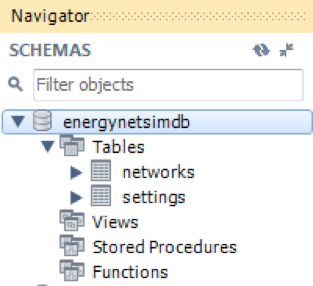
\includegraphics[width=0.4\textwidth]{ErgSoftwareInst4}
	\caption{Das importierte Datenbankschema „energynetsimdb“}
	\label{fig:ErgSoftwareInst4}
\end{figure}
\item [Ausführen der JAR-Datei:] Durch Doppelklick auf die Datei „EnergyNetSim.jar“ wird das Programm gestartet. Im weiteren Verlauf wird die Verwendung des Programmes aus Endanwender-Sicht geschildert.
\end{description}

\subsubsection{Benutzung der Software zum aktuellem Stand}
Da momentan nur das Rahmenwerk für eine spätere Implementierung von Simulationsansätzen realisiert ist, bietet das Programm nur eine eingeschränkte Funktionalität für den Endnutzer. Auf Erweiterungsmöglichkeiten und dafür vorgesehene Strukturen im Kode wird im Anschluss an dieses Kapitel eingegangen.
\begin{figure}[!ht]
	\centering
	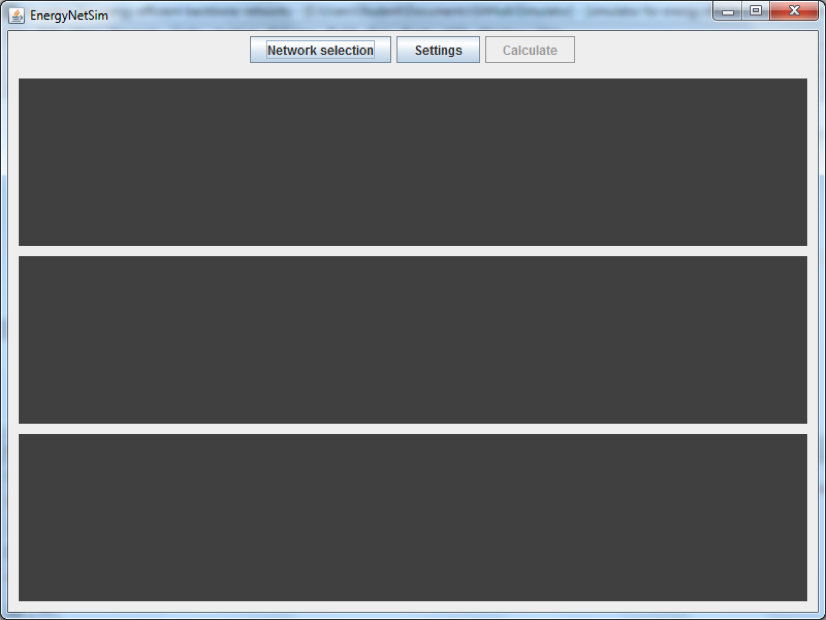
\includegraphics[width=0.6\textwidth]{ErgSoftwareUse1}
	\caption{Hauptfenster nach dem Starten der Software}
	\label{fig:ErgSoftwareUse1}
\end{figure}
Sofern eine Verbindung mit der Datenbank aufgebaut werden konnte, erhält der Benutzer nach Start der Anwendung das Hauptfenster wie in Abbildung 6 angezeigt. Es besteht die Möglichkeit zur Auswahl verschiedener Netze, die in der Datenbank angelegt wurden, über den Menüpunkt „Network selection“ und zur Änderung von Parametern wie beispielsweise dem Strompreis oder dem Netzlastprofil über die Schaltfläche „Settings“.
\begin{figure}[!ht]
	\centering
	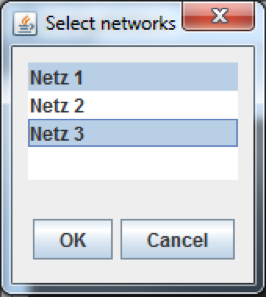
\includegraphics[width=0.2\textwidth]{ErgSoftwareUse2}
	\caption{Dialoge „Select networks“ und „Settings“}
	\label{fig:ErgSoftwareUse2}
\end{figure}
\begin{figure}[!ht]
	\centering
	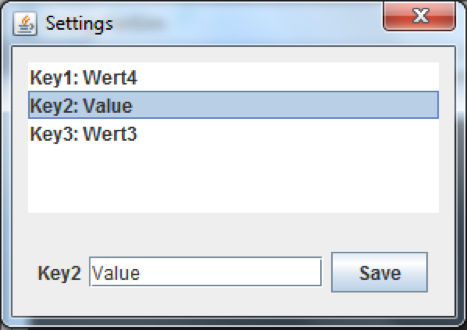
\includegraphics[width=0.4\textwidth]{ErgSoftwareUse3}
	\caption{Dialoge „Select networks“ und „Settings“}
	\label{fig:ErgSoftwareUse3}
\end{figure}
Die geänderten Werte werden in der Datenbank hinterlegt, momentan jedoch von der Kalkulationsmethode nicht weiterverwendet. Stattdessen sind in ihr Werte für den Stromverbrauch, die Netzlast und Kosten hinterlegt, deren Ermittlung in Kapitel \ref{subsec:ErgSch} beschrieben wird.
\begin{figure}[!ht]
	\centering
	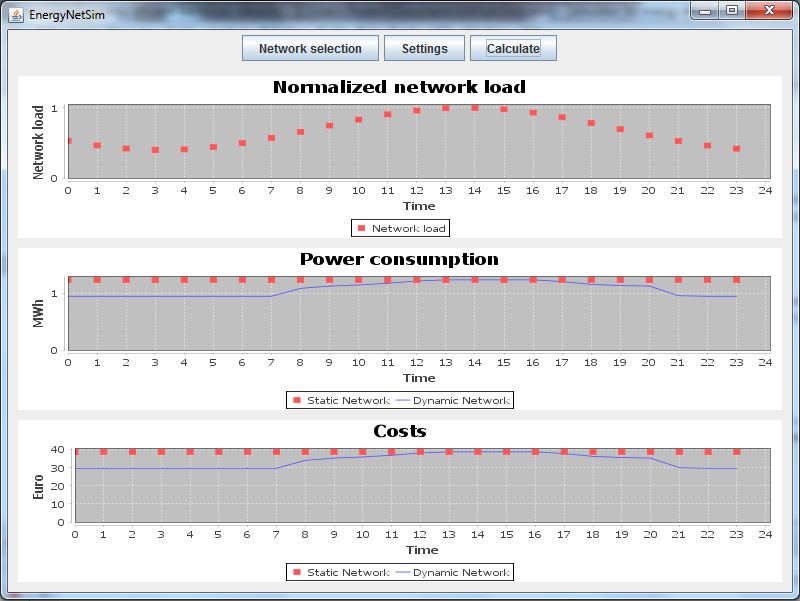
\includegraphics[width=0.8\textwidth]{ErgSoftwareUse4}
	\caption{Ausgabe der Ergebnisse in Diagrammform}
	\label{fig:ErgSoftwareUse4}
\end{figure}
Durch Klick auf die Schaltfläche „Calculate“ werden die Werte in Form von Histogrammen visualisiert.

\subsubsection{Erweiterungsmöglichkeiten} \label{sec:ErgSoftwErweiterung}
Die beschriebene Software stellt freilich keine abgeschlossene Lösung zur Wirtschaftlichkeitsbetrachtung von energieeffizienten Konzepten in simulierten Netzen dar. Wie schon zu Beginn des Kapitels erwähnt, konnte die Entwicklung nicht in der zur Verfügung gestellten Zeit abgeschlossen werden. Vielmehr war die Zielsetzung der Arbeit, eine Anwendung zu erstellen, die es zukünftigen tiefergreifenden Forschungsvorhaben ermöglicht, die fehlenden Algorithmen zu implementieren, welche in Kapitel \ref{subsec:ErgAlg} beschrieben sind, ohne auf Aspekte der grafischen Ausgabe sowie der Anbindung an eine externe Datenbank achten zu müssen.
Das vorliegende Java-Programm erfüllt diese Anforderungen, indem es folgende vordefinierte Methoden und Datenbankstrukturen enthält, die eine Erweiterung um Simulationsalgorithmen zulassen.

\begin{description}
\item [Die Funktion „calculate()“ in der Klasse „MainModel“.] Bei Klick auf die Schaltfläche „Calculate“ wird über den Controller in der Classe „MainModel“ die Funktion „public void calculate()“ aufgerufen. Von dort können der komplette Simulationsalgorithmus gestartet, neue Instanzen von anderen Model-Classen erzeugt und die erhaltenen Ergebnisse in Form einer Liste gespeichert werden.
\item [Das Package „models“.] Das Java-Package „models“ bietet Platz für weitere Klassendefinitionen, die von der „calculate()“-Methode der Klasse „MainModel“ aufgerufen werden und ihrerseits auf die MySQL-Datenbank über die vorhandene Klasse „DatabaseQueries“ zugreifen können. Beispielhaft wurden für die Gerätehardware und die physisch vorhandenen Verbindungen zwischen Knoten die Model-Klassen „HardwareDevices“ und „Link“ angelegt, in denen zukünftig Programmlogik implementiert werden kann.
\item [Das Datenbankschema „energynetsimdb“.] Im Rahmen des Software-Engineering-Prozesses wurde ein Datenbankschema entwickelt, das die Datenstruktur für spätere Simulationsalgorithmen abbilden kann. Das zugehörige Entity-Relationship-Diagramm wurde bereits in Kapitel XX vorgestellt und ermöglicht die Generierung der SQL-Create-Befehle für die noch nicht angelegten Relationen.
\end{description}

Zusammenfassend kann festgestellt werden, dass lediglich Änderungen in der Daten- und Logikschicht innerhalb der bereits vorgegebenen Strukturen durchgeführt werden müssen, um den noch nicht kodierten Simulationsalgorithmus einzubinden. Dazu liegt die vollständige Dokumentation der Software dem Anhang bei.

\subsection{Abschätzung des Energieverbrauchs} \label{subsec:ErgSch}
%Für die zwei Beispiel-Szenarien
% Ausgehend von Kapitel Modellierung
%TODO Verwenden der Werte, die als Dummy Werte in der Software verwendet werden.
% Einbinden auch als Grafik

\section{Diskussion und Erkenntnisse}
%TODO Veronika
% Enthusiasmus und Forschergeist --> Sachlich richtige Simulation entwickeln, um valides Ergebnis zu erreichen
% Algorithmus Entwicklung --> Komplexität und Herausforderungen
% Erkenntnis: Aufgrund der Komplexität (verschiedene Layer, realistische Netzlast (nur "Stream" pro Stunde, keine Berücksichtung von Burst-Traffic, QoS Parameter, Matching der energieeffizienten Konzepte)
% Um die Umsetzbarkeit zu gewährleisten, müssen sehr viele Annahmen getroffen werden (...) --> Ziel des Realismus geht zum Teil verloren.
% Entwicklung des Algorithmus innerhalb der Projektdauer nicht möglich (hier Infos von unten rein nehmen)
% Daher Grundgerüst implementiert und Algorithmus dokumentiert.
% Numerisches Ergebnis der Abschätzung diskutieren. Unterschied deutlich?

Das Ziel des teilweise entwickelten Algorithmus ist das effiziente und realitätsnahe abschätzen der zu erwartenden Energieverbrauchswerte von Backbone-Netzwerken sowohl mit als auch ohne Einsetzen der Energieeinspartechnologien. Es stellte sich während der genaueren Analyse und zu Anfang der Implementierungsphase der Software allerdings heraus, dass der gewählte generische Ansatz einerseits sehr komplex ist und andererseits auf vielen Annahmen und Verallgemeinerungen beruht, die im Vergleich zu echten existierenden Backbone-Netzwerken die Vergleichbarkeit und damit die Praxistauglichkeit der in Entwicklung befindlichen Softwarelösung fast unmöglich machen.
Um die Schwächen des entwickelten Algorithmus auszugleichen oder abzuschwächen ist deutlich mehr Bearbeitungszeit notwendig als für diese wissenschaftliche Arbeit zur Verfügung steht.
Weiterhin zeigt eine Begutachtung der Aufgabenstellung dieser Arbeit, dass die detaillierte Ausarbeitung eines solchen Algorithmus nicht Teil des geforderten oder erwartbarem Umfangs ist.
Aufgrund der genannten Probleme entschieden wir uns dazu, auf die Dokumentation der geleisteten Entwicklung und die Erfüllung der Aufgabenstellung dieser Arbeit den Schwerpunkt zu setzen.


\section{Ausblick}
%
Die diskutierten Ergebnisse machen deutlich, dass eine vollständige Betrachtung der Wirtschaftlichkeit energieeffizienter Netzkonzepte weiterer Forschung bedarf. So wurden im Rahmen der vorliegenden Arbeit nur diejenigen Technologien näher betrachtet, die sich gut in das vereinfachte Netzschema des entwickelten Algorithmus einfügen ließen, und es wurden an vielen Stellen Näherungswerte verwendet.
Die durch die Projektgruppe erarbeiteten Ergebnisse können weitere Forschungsvorhaben vereinfachen. So kann der Programmcode	 als Rahmen zur Implementierung des vorgeschlagenen Algorithmus dienen. Ist die Umsetzung in Java-Code erfolgt, können weitere Konzepte zur Energieeinsparung eingefügt werden. Das entwickelte Datenbankschema kann anschließend verfeinert werden, um schrittweise die zur Vereinfachung des Algorithmus getroffenen Annahmen durch reale Werte zu ersetzen. Schließlich müssen, um die Wirtschaftlichkeit und damit die Attraktivität energieeffizienter Netzkonzepte für die Netzbetreiber vollständig erfassen zu können, auch die Investitionskosten in die Berechnung miteinbezogen werden.
Aufgrund der eingangs erwähnten Entwicklungen hinsichtlich des Wachstums des weltweiten Datenvolumens und der steigenden Energiekosten wird die Betrachtung der Effizienz und Wirtschaftlichkeit energiesparender Netzkonzepte auch in Zukunft ein attraktives Forschungsfeld bleiben.

\newpage
\printbibliography

\end{document}
